
\documentclass[a4paper,11pt]{article}%,twocolumn
%% packages

\usepackage{blindtext} % needed for creating dummy text passages
%\usepackage{ngerman} % needed for German default language
\usepackage{amsmath} % needed for command eqref
\usepackage{amssymb} % needed for math fonts
\usepackage[colorlinks=true,breaklinks]{hyperref} % needed for creating hyperlinks in the document, the option colorlinks=true gets rid of the awful boxes, breaklinks breaks lonkg links (list of figures), and ngerman sets everything for german as default hyperlinks language
\usepackage[hyphenbreaks]{breakurl} % ben�tigt f�r das Brechen von URLs in Literaturreferenzen, hyphenbreaks auch bei links, die �ber eine Seite gehen (mit hyphenation).
\usepackage{xcolor}
\definecolor{c1}{rgb}{0,0,1} % blue
\definecolor{c2}{rgb}{0,0.3,0.9} % light blue
\definecolor{c3}{rgb}{0.3,0,0.9} % red blue
\hypersetup{
    linkcolor={c1}, % internal links
    citecolor={c2}, % citations
    urlcolor={c3} % external links/urls
}
%\usepackage{cite} % needed for cite
\usepackage[square,authoryear]{natbib} % needed for cite and abbrvnat bibliography style
\usepackage[nottoc]{tocbibind} % needed for displaying bibliography and other in the table of contents
\usepackage{graphicx} % needed for \includegraphics 
\usepackage{longtable} % needed for long tables over pages
\usepackage{bigstrut} % needed for the command \bigstrut
\usepackage{enumerate} % needed for some options in enumerate
%\usepackage{todonotes} % needed for todos
\usepackage{makeidx} % needed for creating an index
\makeindex
\usepackage{gensymb}
\usepackage{url}
\usepackage{psfrag}
\usepackage{multirow}
\usepackage{subfigure}
%% page settings

\usepackage[top=20mm, bottom=20mm,left=15mm,right=15mm]{geometry} % needed for page border settings
\parindent=0mm % for space of first line of new text block
\sloppy % for writing with hyphenless justification (tries to)
\hyphenation{} % use hyphenation of tolerance parametershttp://www.jr-x.de/publikationen/latex/tipps/zeilenumbruch.html
\hyphenpenalty=10000
\exhyphenpenalty=10000
\usepackage{fancyhdr} % needed for head and foot options
%% my macros

%% Text fomats
\newcommand{\tbi}[1]{\textbf{\textit{#1}}}

%% Math fonts
\newcommand{\bbA}{\mathbb{A}}
\newcommand{\bbB}{\mathbb{B}}
\newcommand{\bbC}{\mathbb{C}}
\newcommand{\bbD}{\mathbb{D}}
\newcommand{\bbE}{\mathbb{E}}
\newcommand{\bbF}{\mathbb{F}}
\newcommand{\bbG}{\mathbb{G}}
\newcommand{\bbH}{\mathbb{H}}
\newcommand{\bbI}{\mathbb{I}}
\newcommand{\bbJ}{\mathbb{J}}
\newcommand{\bbK}{\mathbb{K}}
\newcommand{\bbL}{\mathbb{L}}
\newcommand{\bbM}{\mathbb{M}}
\newcommand{\bbN}{\mathbb{N}}
\newcommand{\bbO}{\mathbb{O}}
\newcommand{\bbP}{\mathbb{P}}
\newcommand{\bbQ}{\mathbb{Q}}
\newcommand{\bbR}{\mathbb{R}}
\newcommand{\bbS}{\mathbb{S}}
\newcommand{\bbT}{\mathbb{T}}
\newcommand{\bbU}{\mathbb{U}}
\newcommand{\bbV}{\mathbb{V}}
\newcommand{\bbW}{\mathbb{W}}
\newcommand{\bbX}{\mathbb{X}}
\newcommand{\bbY}{\mathbb{Y}}
\newcommand{\bbZ}{\mathbb{Z}}
\usepackage[ framed, numbered]{matlab-prettifier}%framed,%
\usepackage{listings}
\usepackage{physics}
\usepackage{pdfpages}
\usepackage[toc,page]{appendix}
\usepackage{float}
\usepackage{hyperref}

% for code
\usepackage{listings}
\usepackage{color}
% Define colors
\definecolor{codegreen}{rgb}{0,0.6,0}
\definecolor{codegray}{rgb}{0.5,0.5,0.5}
\definecolor{codepurple}{rgb}{0.58,0,0.82}
\definecolor{backcolour}{rgb}{0.95,0.95,0.92}
% Setup the listings package
\lstset{
    backgroundcolor=\color{backcolour},   
    commentstyle=\color{codegreen},
    keywordstyle=\color{magenta},
    numberstyle=\tiny\color{codegray},
    stringstyle=\color{codepurple},
    basicstyle=\footnotesize,
    breakatwhitespace=false,         
    breaklines=true,                 
    captionpos=b,                    
    keepspaces=true,                 
    numbers=left,                    
    numbersep=5pt,                  
    showspaces=false,                
    showstringspaces=false,
    showtabs=false,                  
    tabsize=2
}

\newenvironment{qanda}{\setlength{\parindent}{0pt}}{\bigskip}
\newcommand{\Q}{\bigskip\bfseries Q: }
\newcommand{\A}{\par\textbf{Answer: } \normalfont}

\begin{document}
\begin{titlepage}
\center % Center everything on the page

%-------------------------------------------------------------------------------------
%	HEADING SECTIONS
%------------------------------------------------------------------------------------
\textbf{\large Department of Electrical and Computer Engineering}\\[0.5cm]
\textbf{\Large University of Colorado at Boulder}\\[1cm]
\textbf{\large ECEN5623 - Real Time Embedded Systems }\\[2cm]

\includegraphics[width=0.3\textwidth]{figures/cu}\\[2cm]

	
%-------------------------------------------------------------------------------------
%	TITLE SECTION
%------------------------------------------------------------------------------------
\textbf{\Huge Exercise 5 }\\[0.2cm]



%----------------------------------------------------------------------------------------
%	MEMBERS SECTION
%----------------------------------------------------------------------------------------


\vfill

\textbf{\large Submitted by}\\[0.5cm]

{\large Parth | Jithedra}\\[0.5cm]	

%----------------------------------------------------------------------------------------
%	DATE SECTION
%----------------------------------------------------------------------------------------

\textbf{\large Submitted on}
\textbf{\Large \today} % Date, change the \today to a set date if you want to be precise

%----------------------------------------------------------------------------------------

\vfill % Fill the rest of the page with whitespace

\end{titlepage}


\pagebreak

\tableofcontents
\listoffigures
\listoftables
\vfill
\begin{center}
	\textbf{\textit{*PDF is clickable}}
\end{center}

\pagebreak

\section*{Objective}
\begin{enumerate}
	\item Understanding the concept of the Cyclic Executive in comparison to Linux POSIX RT threading and RTOS.
	      Implementing and analyzing custom feasibility test code for different scheduling policies (RM, EDF, LLF) using Cheddar.
	\item Moreover, understanding the constraints, assumptions, and derivation steps in Rate Monotonic (RM) Least Upper Bound (LUB) as outlined in Chapter 3 of the textbook.

\end{enumerate}

\pagebreak
\begin{qanda}
	\section{Question 1}
	\begin{enumerate}
		\item[] \Q [5 points] make yourself an account on your Dev Kit.
			\begin{enumerate}
				\addcontentsline{toc}{subsection}{A}
				\item \Q enable SSH via the GUI or with
				      headless methods.

				      \A To enable SSH on the Jetson Nano, either through the graphical user interface (GUI) or headlessly, follow these steps:
				      \begin{enumerate}
					      \item \textbf{Connecting the Device:} First, connect the Jetson Nano to your computer using a USB cable. This establishes a virtual Ethernet connection between your PC and the Nano.
					      \item \textbf{Finding the IP Address:} Use the ipconfig command on Windows or ifconfig on Linux/Mac to list all network devices and their configurations. Look for an entry related to the Nano, which should show an IP address assigned by DHCP.
					      \item \textbf{Identifying the Gateway IP:} To find the gateway IP address, use the arp -a command. This command displays the ARP table, which includes the IP addresses of all devices on the network. In this case, you found the gateway IP to be 192.168.55.1.
					      \item \textbf{SSH into the Nano:} With the gateway IP identified, you can SSH into the Jetson Nano using its IP address and your username. The command format is ssh username@ip\_address, so in my case, it would be ssh parthishere@192.168.55.1
					      \item Screenshot for SSH connection
					            \begin{figure}[H]
						            \centering
						            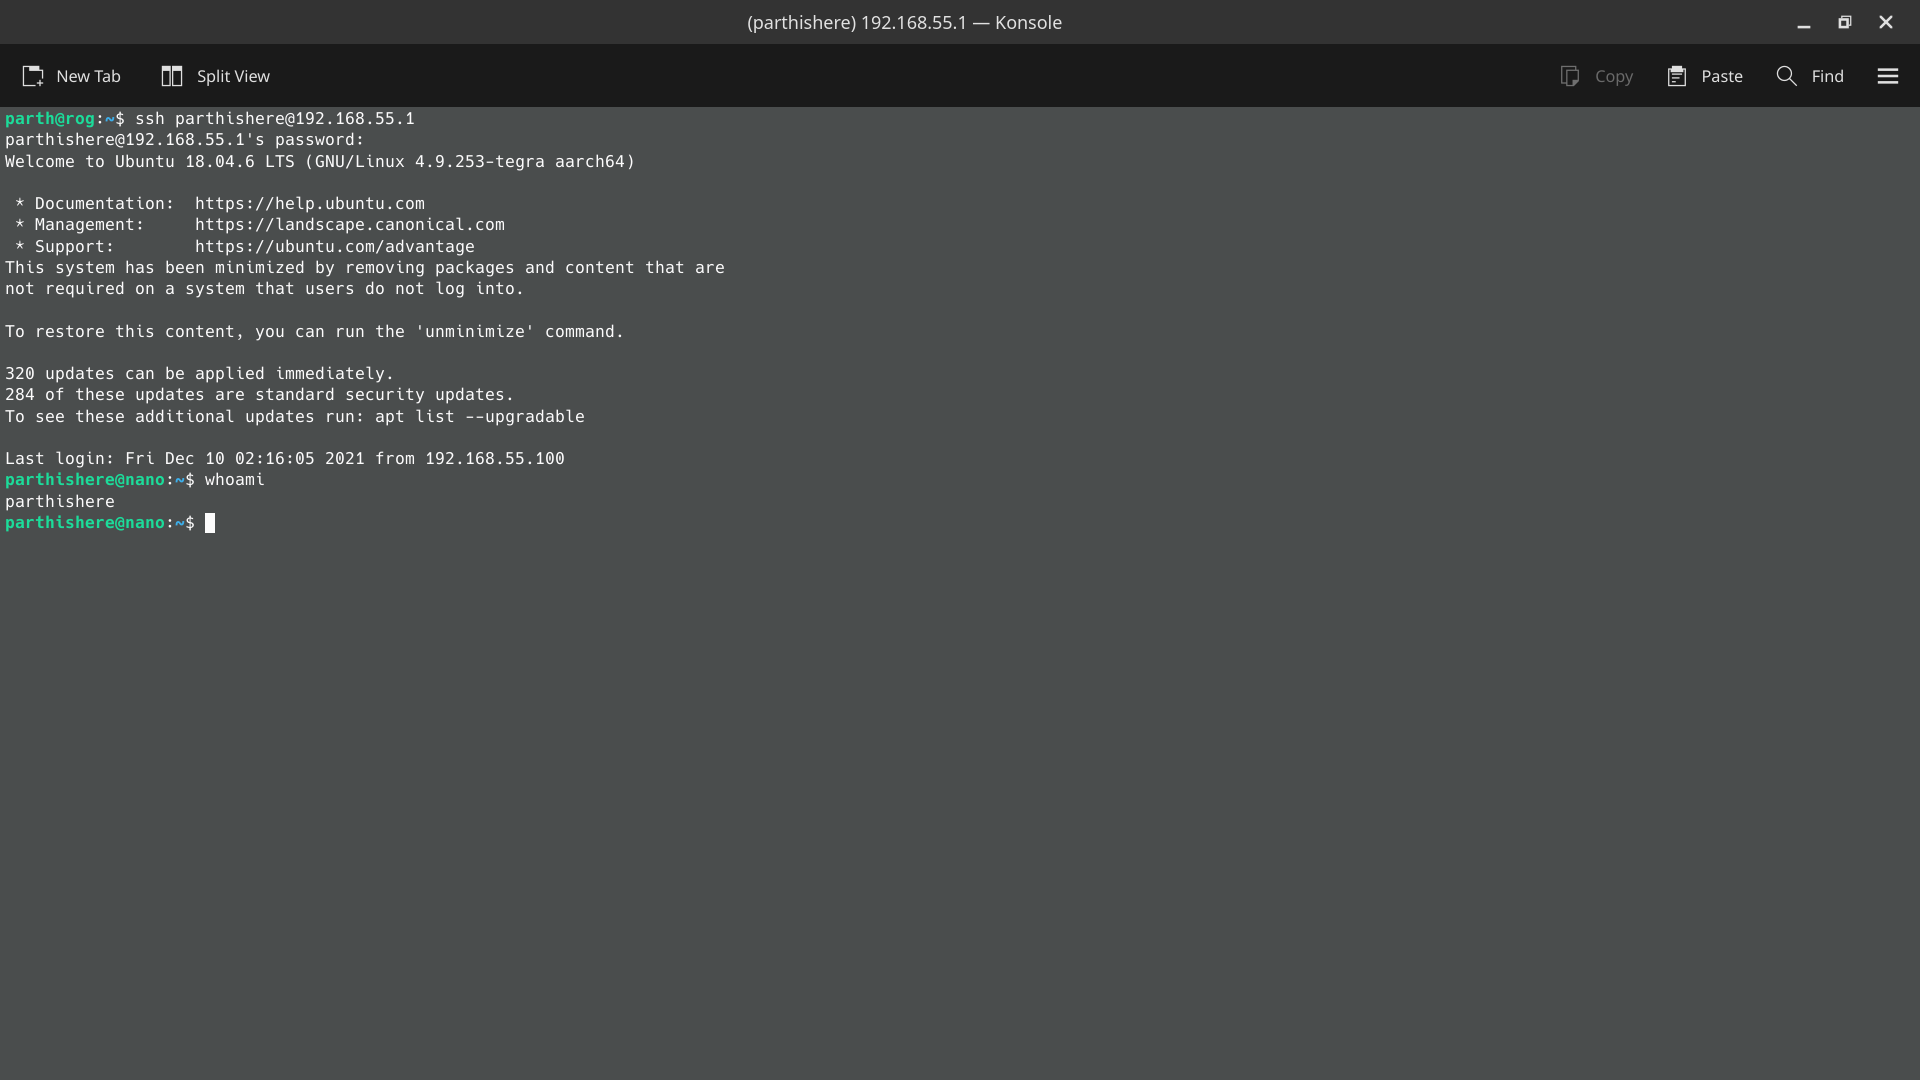
\includegraphics[scale=0.32]{figures/ssh.png}
						            \caption{SSH connection with jatson nano}
					            \end{figure}

				      \end{enumerate}



				      To set up VNC on the Jetson Nano for remote desktop access:

				      \begin{enumerate}
					      \item Editing Vino Settings: Open the Vino settings file for editing with
					            \begin{lstlisting}[language=bash]
sudo nano /usr/share/glib-2.0/schemas/org.gnome.Vino.gschema.xml.
\end{lstlisting}

					      \item Modifying the XML File: Insert the following XML key to enable remote desktop access through VNC:
					            \begin{lstlisting}[language=bash]
<key name='enabled' type='b'>
	<summary>Enable remote access to the desktop</summary>
		<description>
			If true, allows remote access to the desktop via the RFB protocol. 
			Users on remote machines may then connect to the desktop using a 
			VNC viewer.
		</description>
	<default>true</default>
</key>
\end{lstlisting}

					      \item Compiling Schemas: After adding the key, compile the schemas with sudo glib-compile-schemas /usr/share/glib-2.0/schemas.

					      \item Adjusting Vino Settings: Disable encryption and the prompt for VNC connections by running:
					            \begin{lstlisting}[language=bash]
gsettings set org.gnome.Vino require-encryption false
gsettings set org.gnome.Vino prompt-enabled false
\end{lstlisting}
					      \item Enabling Vino Server: Reload the system daemon and enable the Vino server for VNC access using:

					            \begin{lstlisting}[language=bash]
systemctl daemon-reload
systemctl enable /usr/lib/vino/vino-server
\end{lstlisting}
					      \item After setting up VNC on the Nano and identifying the IP address via arp -a, you can use a VNC viewer downloaded from the internet to connect to the Nano for remote desktop access.
				      \end{enumerate}



				      \begin{figure}[H]
					      \centering
					      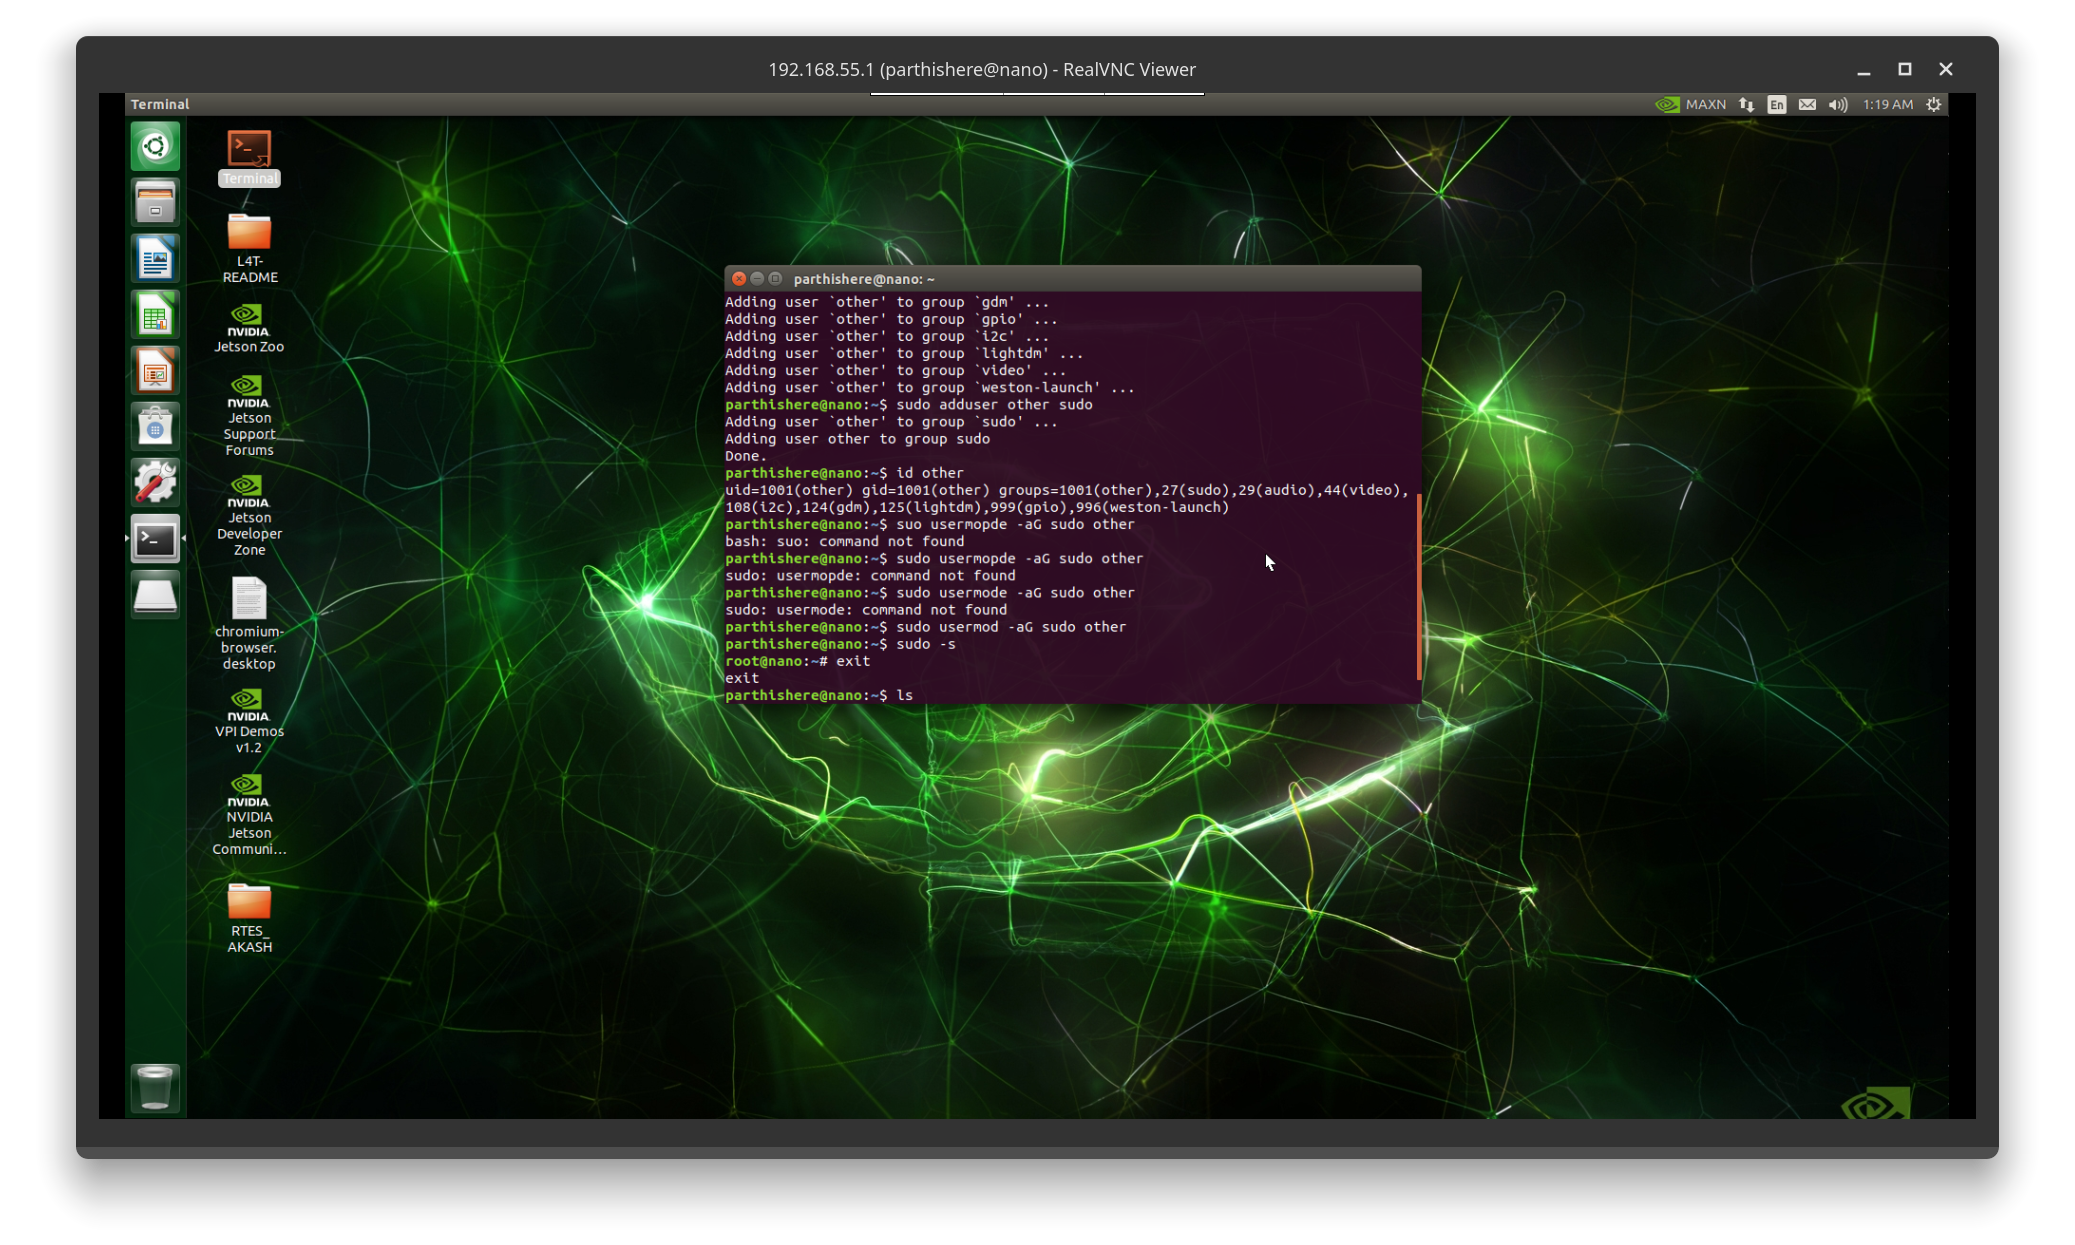
\includegraphics[scale=0.32]{figures/vnc.png}
					      \caption{VNC(user creation and showing)}
				      \end{figure}

				      \begin{figure}[H]
					      \centering
					      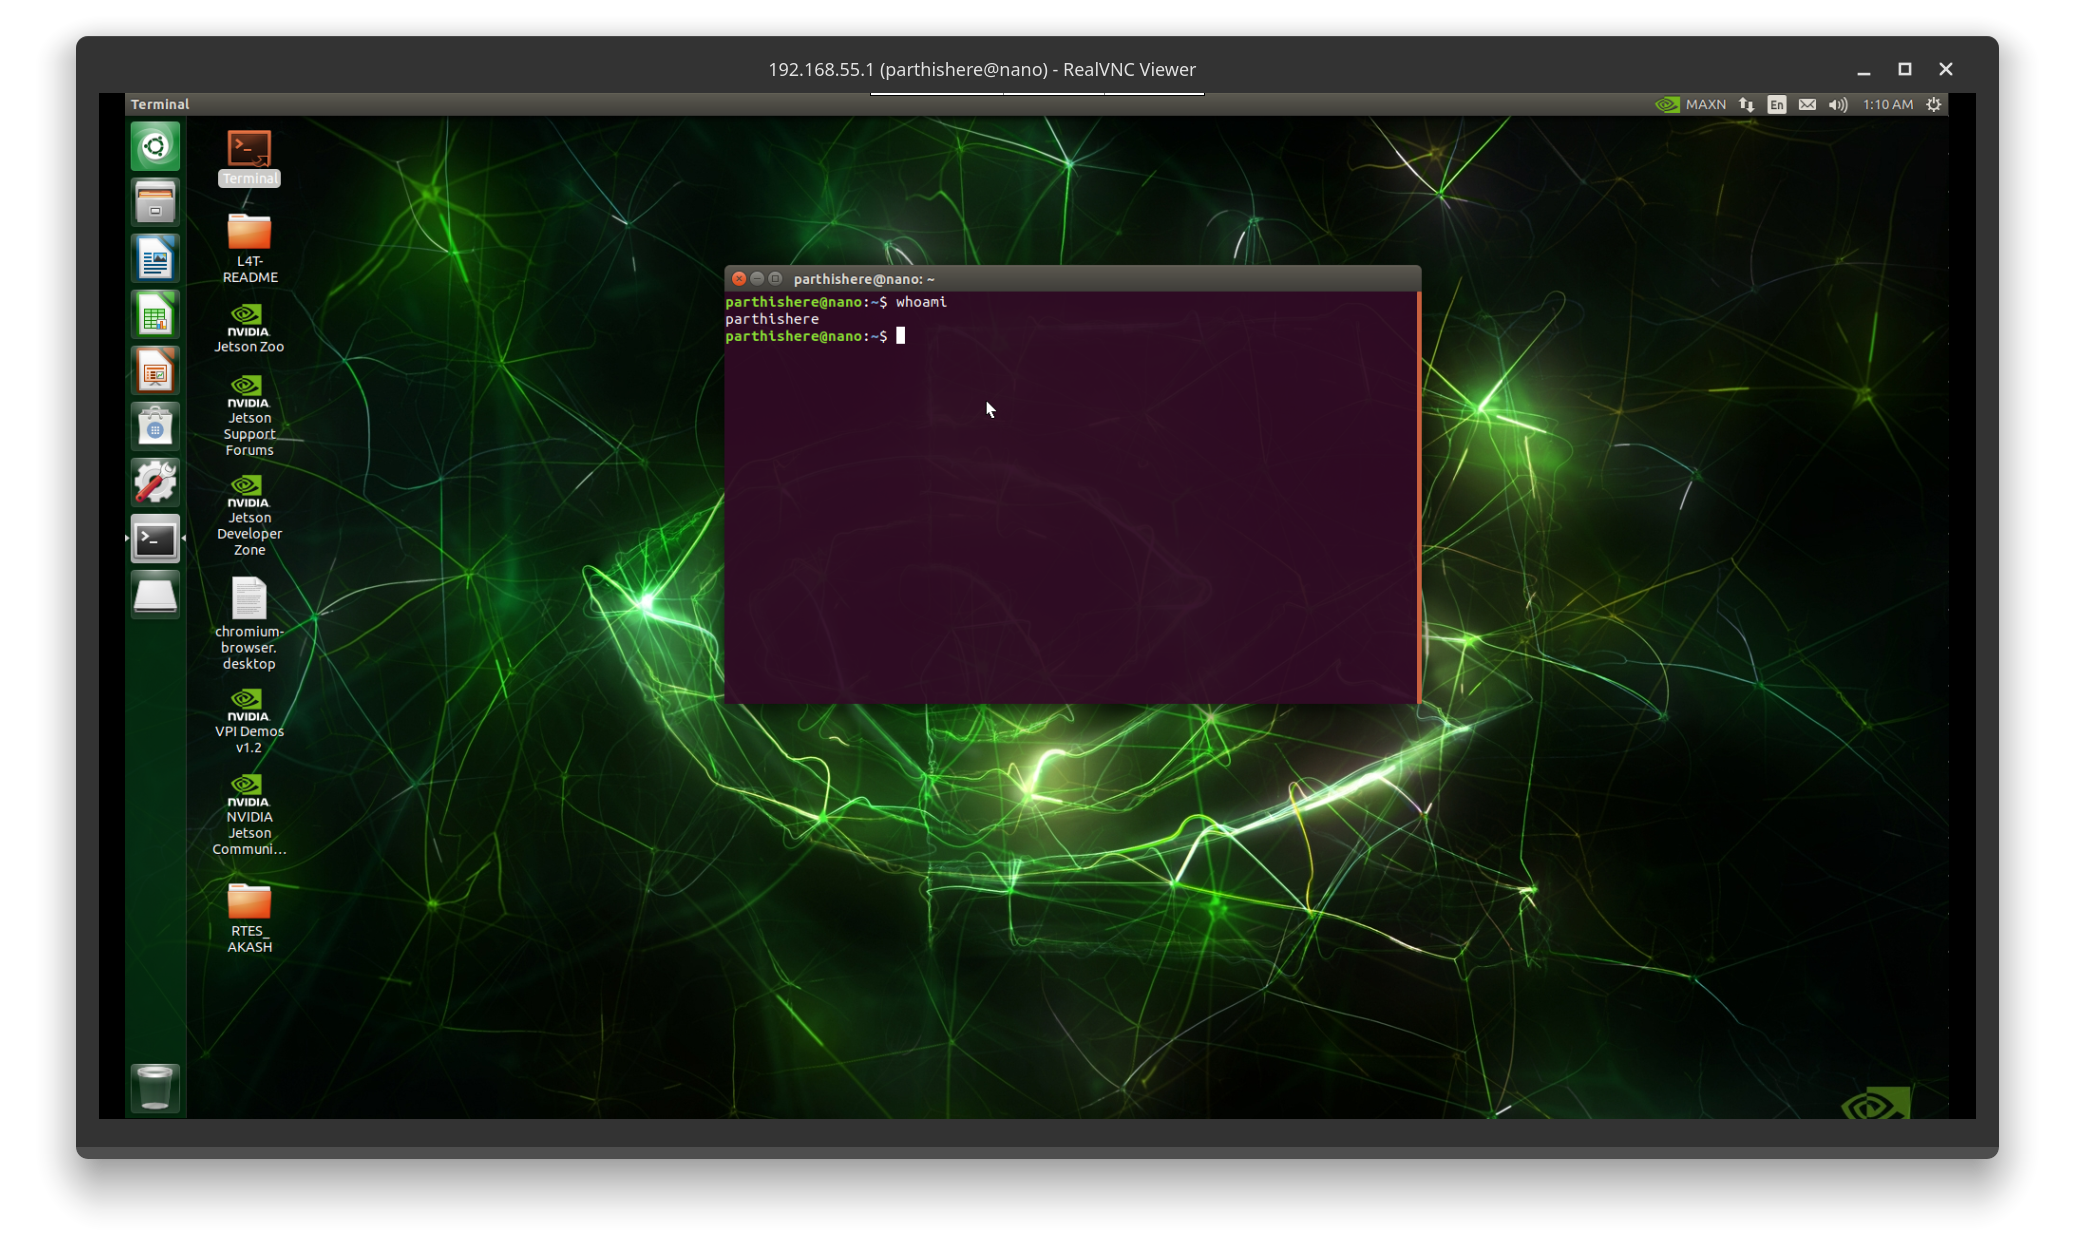
\includegraphics[scale=0.32]{figures/vnc2.png}
					      \caption{VNC }
				      \end{figure}

				      \addcontentsline{toc}{subsection}{B}
				\item \Q  Show evidence that you have created a custom login with screenshots or photos from your phone.

				      \A We can see the title bar of my PC showing VNC viewer for the screen of jatson nano
				      \begin{figure}[H]
					      \centering
					      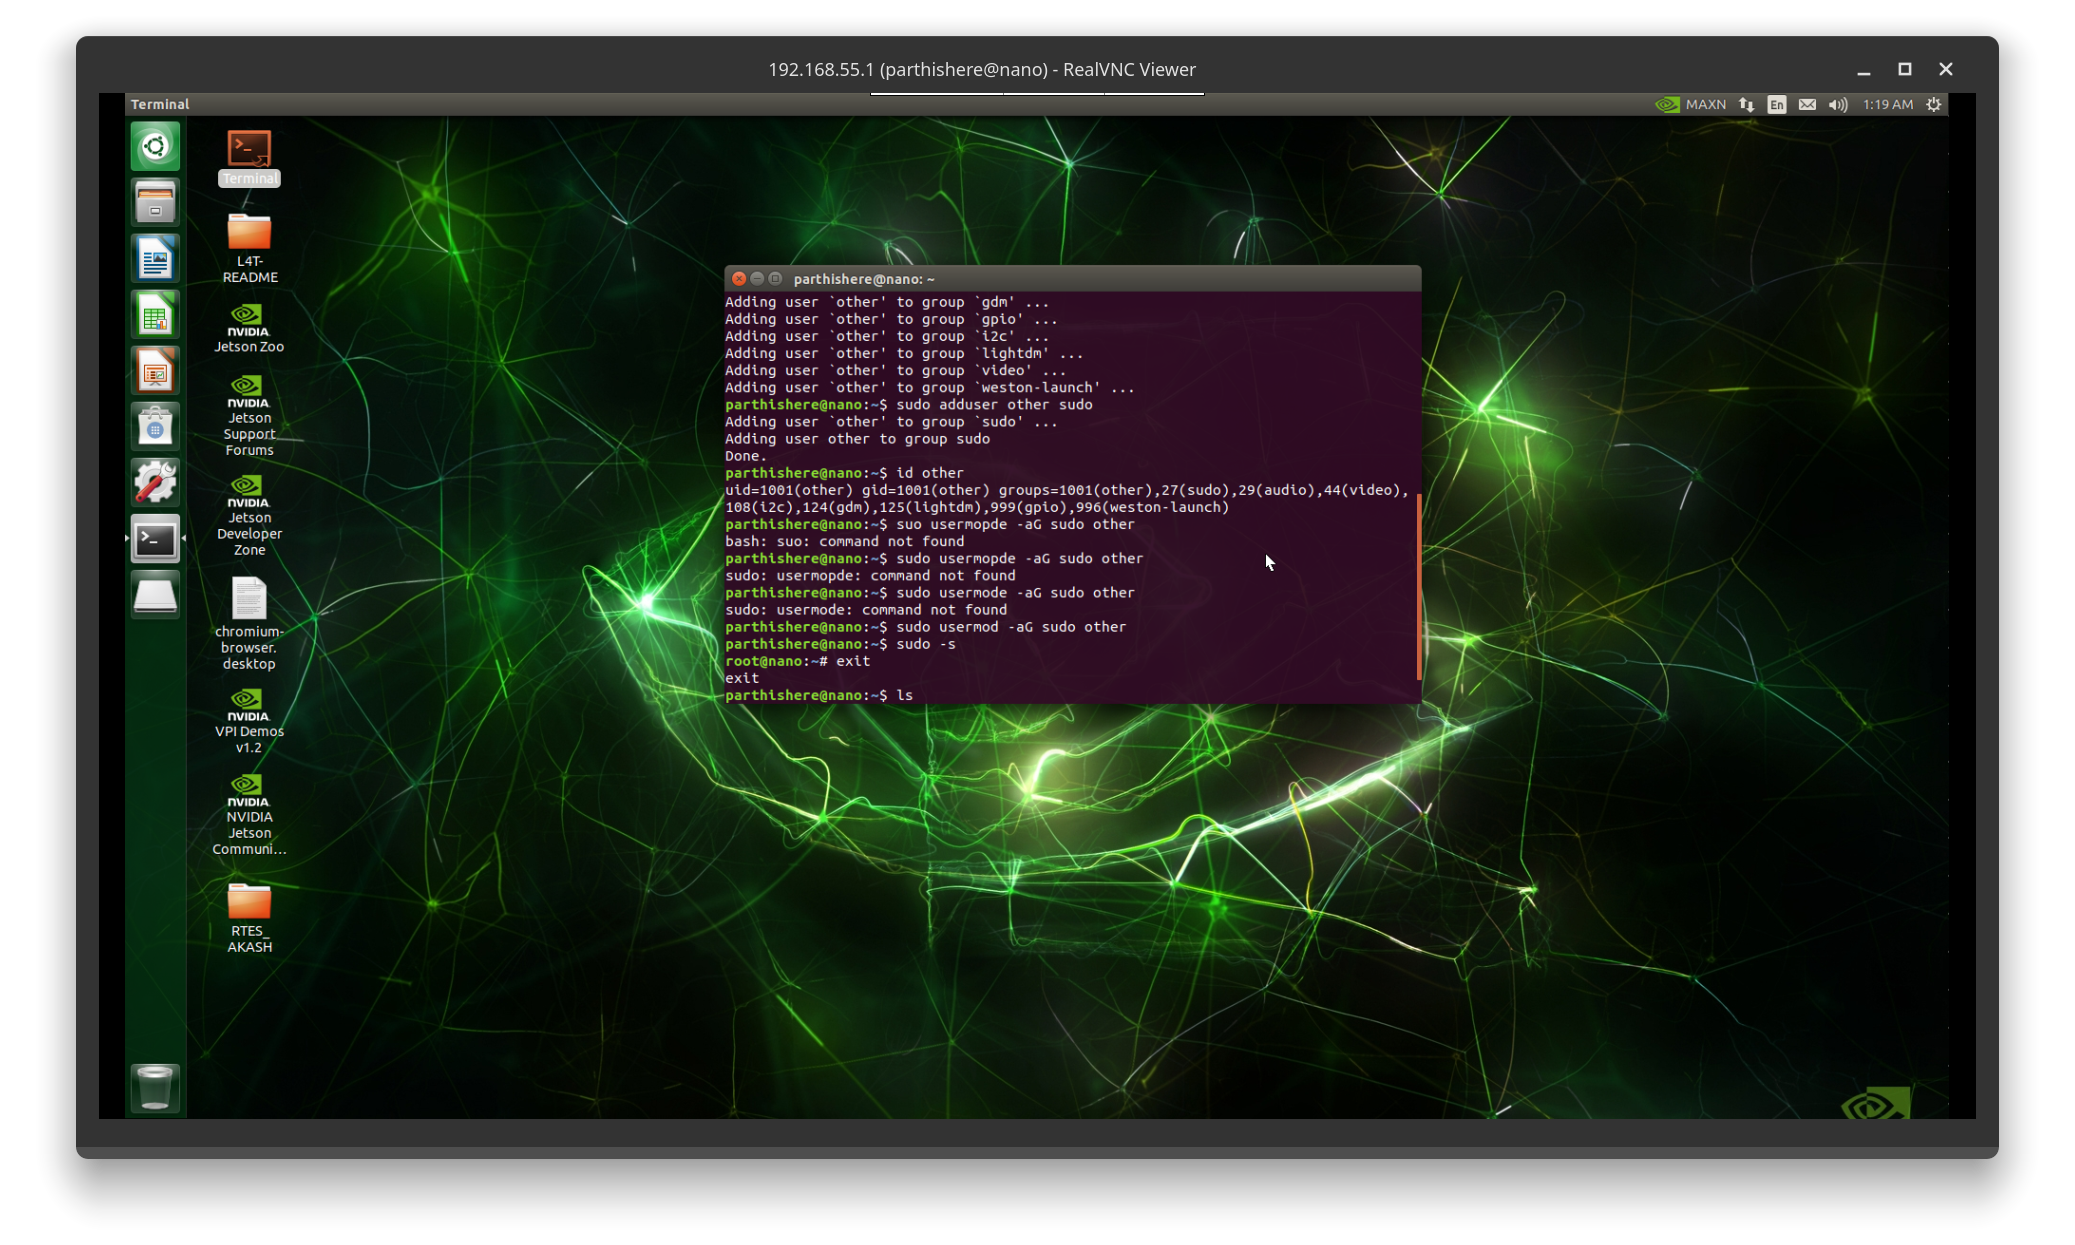
\includegraphics[scale=0.32]{figures/vnc.png}
					      \caption{VNC(user creation and showing)}
				      \end{figure}



			\end{enumerate}


	\end{enumerate}




	\section{Question 2}
	\begin{enumerate}
		\item[] \Q [10 points] Read the paper "Architecture of the Space Shuttle Primary Avionics Software
			System", by Gene Carlow.
			\begin{enumerate}
				\addcontentsline{toc}{subsection}{A}
				\item \Q Provide an explanation and critique of the frequency executive architecture.

				      \A
				      \begin{itemize}
					      \item The Frequency Executive architecture described in the ”Architecture of the Space Shuttle Primary Avionics Software System” by Gene Carlow is central to the Guidance, Navigation, and Control GN\&C design structure
					            of the Space Shuttle’s Primary Avionics Software System PASS.
					      \item The on-board software is based on three applications.
					      \item One among them is GN\&C(Guidance, navigation and control) software.
					      \item It is used to determine vehicle position, velocity and altitude.
					      \item There are two modules in GN\&C Design structure - Cyclic and Non-Cyclic Module.
				      \end{itemize}

				 
				      \begin{figure}[H]
					      \centering
					      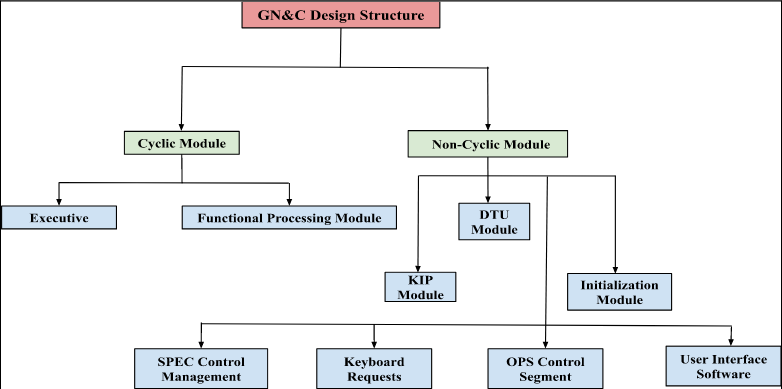
\includegraphics[scale=0.7]{figures/fea.png}
					      \caption{Frequency executive architecture}
				      \end{figure}

				      \begin{itemize}
					      \item OPS Control Segment : The control segment initiates a repeating set of tasks, and the FCOS(Fixed Cycle
					            Offset Scheduling) scheduling method, facilitated by a Supervisor Call, plays a role in managing and executing
					            these tasks.
					      \item \textbf{Executive :}
					            \begin{itemize}
						            \item It is a cyclic process that is used to control the starting and managing the timing and synchronizing the	principal functions and I/Os.
						            \item It involves managing the phasing and sequencing between significant operational modes and the OPS
						                  through a Dispatcher Table Update (DTU) module.
						            \item This strategy enables flexible control and modification of the execution sequence of primary functions, accommodating dynamic adjustments as required.

					            \end{itemize}

					      \item There are three executive structures those are integrated into the Guidance, Navigation, and Control \(GN\&C\) design to ensure the timely completion of critical flight control processing within a 40-millisecond minor cycle.
					      \item The high-frequency executive operates at a priority level that enables it to cycle at a rate of 25 Hz, initiating	principal functions directly linked to vehicle flight control.
					      \item Additionally, mid-frequency and low-frequency executives, scheduled at lower priorities, initiate principal function processes with the rates ranging from 6.25 Hz to 0.25 Hz.
				      \end{itemize}

				      \begin{figure}[H]
					      \centering
					      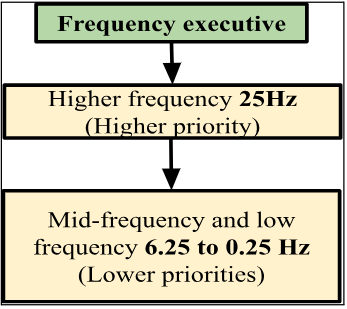
\includegraphics[scale=0.7]{figures/ce2.png}
					      \caption{Frequency executive architecture}
				      \end{figure}

				      \begin{itemize}
					      \item \textbf{SPEC Control Management :}
					            \begin{itemize}
						            \item The OPS substructure includes a second element known as the specialist function (SPEC).
						            \item Unlike major modes, SPEC is used for secondary functions and is activated within an OPS only in
						                  response to a keyboard entry by the crew.
						            \item After initialization, SPEC runs independently and concurrently with other processing within the OPS.
					            \end{itemize}

					      \item \textbf{Initialization Module :} Loading and initialization are performed by the System Control.
					      \item \textbf{Keyboard Requests :}
					      \item \begin{itemize}
						            \item Communication links are formed between the keyboard/display units and the avionic subsystems they
						                  support throughout the execution of all Operational Sequences (OPSs).
						            \item A recurrent procedure is initiated at the systems level to ensure system integrity.
						            \item This process establishes the 40-millisecond timing cycle that is fundamental to the avionic system
						                  architecture and guarantees consistent service to these interfaces.
					            \end{itemize}

					      \item \textbf{User Interface Software :} The user interface software manages communication between users and various systems or applications, overseeing intercomputer communication and ensuring redundant computer
					            synchronization as part of the systems software.
				      \end{itemize}



				      \addcontentsline{toc}{subsection}{B}
				\item \Q What advantages and disadvantages does the frequency executive have compared to the real-time threading and tasking implementation methods for real-time software systems?	Please be specific about the advantages and disadvantages and provide at least 3 advantages as well as 3 disadvantages.
				      \A
				      Advantages
				      \begin{enumerate}
					      \item \textbf{Predictability and Determinism:} The cyclic priority scheduling of the Frequency Executive ensure that critical tasks are executed within predictable time frames, which is essential for the real-time requirements of spacecraft control. This predictability provides a high level of determinism in system behavior.

					      \item \textbf{Modularity and Flexibility:} The use of a table-driven dispatching design allows for flexibility in modifying the sequencing of tasks as mission requirements change, without the need for significant code changes. This modularity supports the adaptability of the software to different phases of a space mission and facilitates updates and maintenance.

					      \item \textbf{Efficient Resource Utilization:} By dividing tasks based on their frequency requirements and assigning them to different executives, the architecture enables efficient utilization of computing resources. This approach helps in managing the limited computational capacity of onboard systems by ensuring that high-priority tasks have the resources they need when they need them.\\
				      \end{enumerate}

				      Disadvantages
				      \begin{enumerate}
					      \item \textbf{Complexity in Management and Scheduling:} While the Frequency Executive architecture offers flexibility and predictability, it also introduces complexity in the management and scheduling of tasks. Developers need to carefully plan and coordinate the execution frequencies and priorities of tasks to avoid conflicts and ensure that all tasks meet their timing requirements.

					      \item \textbf{Limited Scalability:} As the number of tasks and their complexity grow, managing them within the constraints of the Frequency Executive architecture can become challenging. The fixed cyclic nature and the need for predefined scheduling tables may limit scalability and the ability to dynamically adjust to unforeseen operational demands.

					      \item \textbf{Potential for Resource Under-Utilization:} While the architecture is to optimize resource utilization, the fixed scheduling can lead to periods where computational resources are underutilized, if tasks do not align perfectly with the executive cycles. This inefficiency could be a drawback in scenarios where maximizing computational throughput is critical.
				      \end{enumerate}

			\end{enumerate}


	\end{enumerate}




	\section{Question 3}
	\begin{enumerate}
		\item[] \Q  [5 points] Read the paper “Building Safety-Critical Real-Time Systems with Reuseable
			Cyclic Executives”, available from http://dx.doi.org/10.1016/S0967-0661(97)00088-9. In
			other embedded systems classes you built ISR (Interrupt Service Routine) processing
			software and polling/control loops to control for example stepper motors – describe the
			concept of the Cyclic Executive and how this compares to the Linux POSIX RT threading
			and RTOS approaches we have discussed.
			\A

			\textbf
			\textbf{The Cyclic Executive}
			\begin{enumerate}
				\item[] \textbf{Concept:} The Cyclic Executive is a simple and deterministic scheduling method primarily used in hard real-time systems. It operates on a fixed schedule known as a major cycle, divided into minor cycles. Each minor cycle is further divided into frames, with each frame allocated to a specific task or a set of tasks. The tasks are executed in a predefined sequence, repeating in every major cycle. This approach eliminates the need for dynamic task scheduling, as the execution pattern is statically determined during the system design phase.

					\begin{figure}[H]
						\centering
						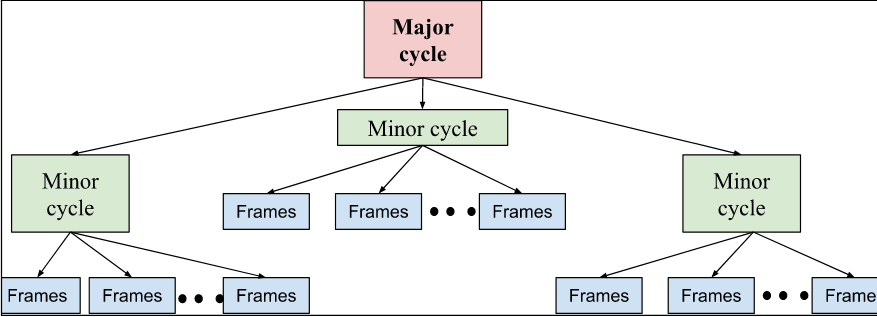
\includegraphics[scale=0.7]{figures/ce.png}
						\caption{Cyclic Executive}
					\end{figure}

					\textbf{Scheduling Structure:}
					\begin{enumerate}
						\item \textbf{Major Cycle:} Represents the highest-level schedule, defining the sequence of processes that execute during a major cycle. This sequence cyclically repeats until the system's operating mode changes.
						\item \textbf{Minor Cycle:} Divides the major cycle into smaller units, and each tick of the minor cycle clock indicates the end of a minor cycle. Synchronization is enforced by the ticks of the minor cycle clock, ensuring that real-time requirements are met. Minor cycle clock ticks indicate the end of a minor cycle, and processes must complete their execution within this timeframe to avoid minor cycle overruns.
						\item \textbf{Frame:} Within each minor cycle, frames further divide the schedule. Only one process in the sequence	corresponding to the minor schedule executes within a frame.
					\end{enumerate}



			\end{enumerate}


			\textbf{Interrupt Service Routine (ISR):}
			In embedded systems, ISRs are commonly used to handle hardware interrupts and time-sensitive tasks.
			In Linux RT, ISRs can be implemented using kernel threads or dedicated real-time threads with high priority

			\textbf{Linux POSIX RT Threading}
			\begin{enumerate}
				\item[] \textbf{Concept:} POSIX RT threading in Linux provides a set of standardized APIs for developing real-time applications within a general-purpose operating system environment. It includes features for creating real-time threads, setting thread priorities, and employing synchronization mechanisms like mutexes and condition variables.

					\item[]\textbf{Characteristics:}

					\textbf{Preemptive Multitasking:} Higher-priority threads can preempt lower-priority ones, allowing urgent real-time tasks to interrupt less critical tasks.
					\textbf{Concurrency:} Supports the concurrent execution of multiple threads, facilitating complex real-time applications.
					\textbf{Non-Deterministic Overheads:} Running atop a general-purpose OS, POSIX RT threads may encounter non-deterministic behaviors due to OS overheads and other system activities
			\end{enumerate}


			\textbf{Comparison}
			\begin{table}[H] % 'h' here means 'here', place the table approximately here
				\centering
				\caption{Comparison Table}
				\label{table:multiline}
				\begin{tabular}{|l|p{4cm}|p{4cm}|p{4cm}|}
					\hline
					\textbf{}                    & \textbf{Cyclic Executive}                   & \textbf{RTOS}                                                   & \textbf{Linux POSIX with Real-Time Services}                           \\
					\hline
					\textbf{Primary Usage}       & Deeply embedded systems (eg.shuttle flight) & Embedded systems, scalable and portable (eg. Vx Works) & General-purpose systems with real-time needs (eg. concurrent) \\
					\hline
					\textbf{Scheduling approach} & Custom, fixed sequence.                     & Preemptive and cooperative scheduling                  & Preemptive scheduling with real-time extensions               \\
					\hline
					\textbf{Task Management}     & Limited or none                             & Comprehensive task management                          & Supports multitasking and task synchronization                \\
					\hline
					\textbf{Overhead}            & Low                                         & Medium                                                 & High                                                          \\
					\hline
					\textbf{Maintenance}         & Costly due to hard coding                   & Simpler maintenance due to task abstractions           & Requires constant updates, higher maintenance                 \\
					\hline
					\textbf{Flexibility}         & Highly custom, efficient                    & Moderate flexibility                                   & High flexibility applications                                 \\
					\hline
					\textbf{Licensing}           & Usually free or low	cost.                    & Licensing costs may apply                              & Licensing costs may apply, open-source options available      \\
					\hline
					\textbf{Developement time}   & Longer development time                     & Quick                                                  & Balanced, quicker than cyclic	executive, slower than RTOS      \\
					\hline
				\end{tabular}
			\end{table}

	\end{enumerate}

	\pagebreak
	\section{Question 4}
	\begin{enumerate}
		\item[] \Q [50 points] CUSTOM FEASIBLITY TEST CODE. Download Feasibility example code (or
			get it from Canvas) and build it on a Jetson, Raspberry Pi, DE1-SoC or TIVA or Virtual Box
			and execute the code.
			\begin{enumerate}
				\addcontentsline{toc}{subsection}{A}
				\item \Q  Compare the feasibility tests provided by the example code to analysis using Cheddar for
				      the first 5 examples (0-4).
				      \A

				      \begin{enumerate}
					      \addcontentsline{toc}{subsubsection}{Example 0}
					      \item \textbf{Example 0}
					            \begin{enumerate}
						            \item \textbf{Cheddar Output:}\\

						                  \begin{figure}[H]
							                  \centering
							                  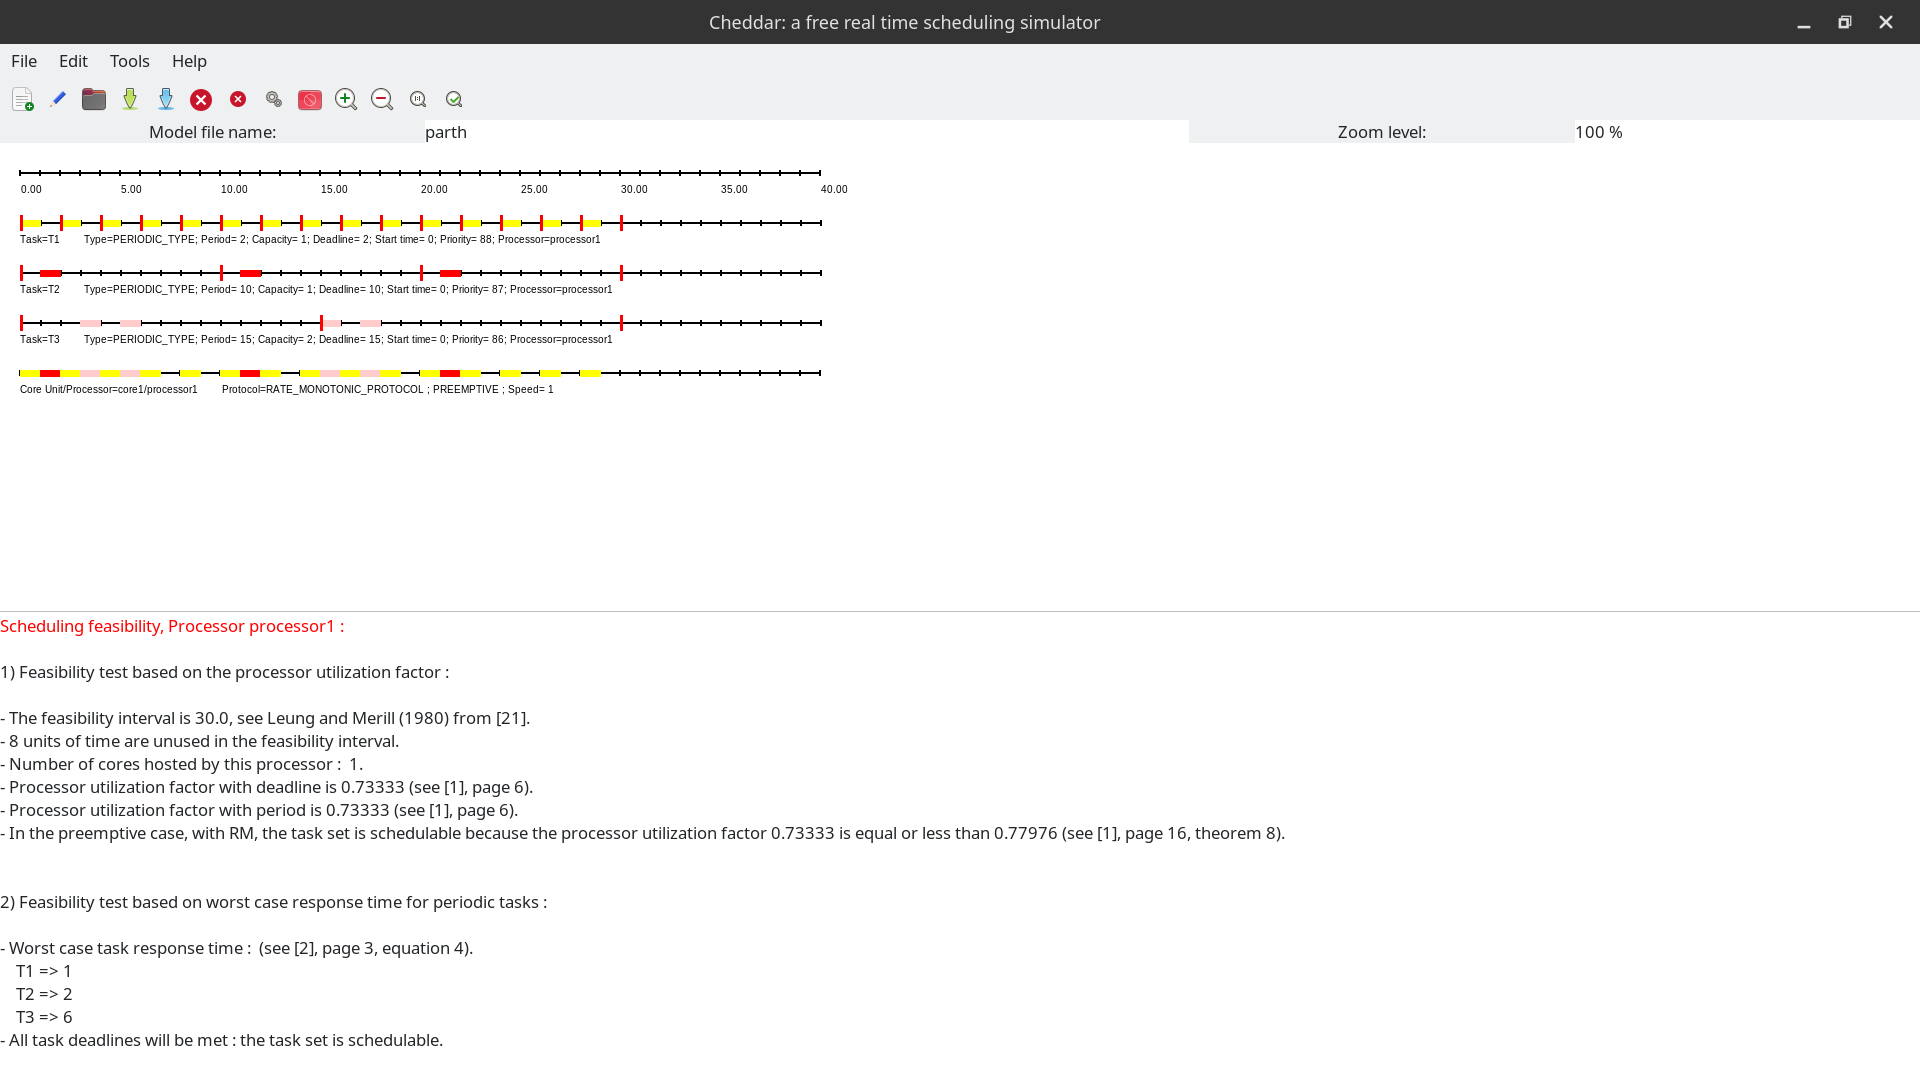
\includegraphics[scale=0.36]{figures/exmaple0_rm.png}
							                  \caption{Example 0, RM test}
						                  \end{figure}
						            \item \textbf{Code Output:}\\
						                  \begin{verbatim}
****************
Example 0
C: 1 1 2
T: 2 10 15
D: 2 10 15

Task 0, WCET=1, Period=2, Utility Sum = 0.500000
Task 1, WCET=1, Period=10, Utility Sum = 0.600000
Task 2, WCET=2, Period=15, Utility Sum = 0.733333

Total Utility Sum = 0.733333
LUB = 0.779763
RM LUB: Feasible
Completion time feasibility: Feasible
Scheduling point feasibility: Feasible
\end{verbatim}
						            \item \textbf{Conclusion:}\\
						                  We found out that the Least Upper Bound (LUB) is 0.779763, both in our calculations and using the Cheddar tool, so our results match perfectly. The CPU usage we worked out is about 73.33\%, and this number is the same when we look at how much of the CPU is used in the Cheddar tool, considering the time tasks take and their deadlines.\\

						                  Because the LUB value is higher than the actual CPU usage RM\_LUB would fail in the test, but all our checks for nessesarry and sufficient tests Completion time and Scheduling point feasibility shows that the tasks are feasible with RM schedule. This means we set up our tasks in a way that they can all get done within their set times without overloading the CPU. And we can confirm the results of no deadline miss in the cheddar.

					            \end{enumerate}
					            \addcontentsline{toc}{subsubsection}{Example 1}
					      \item \textbf{Example 1}
					            \begin{enumerate}
						            \item \textbf{Cheddar Output:}\\
						                  \begin{figure}[H]
							                  \centering
							                  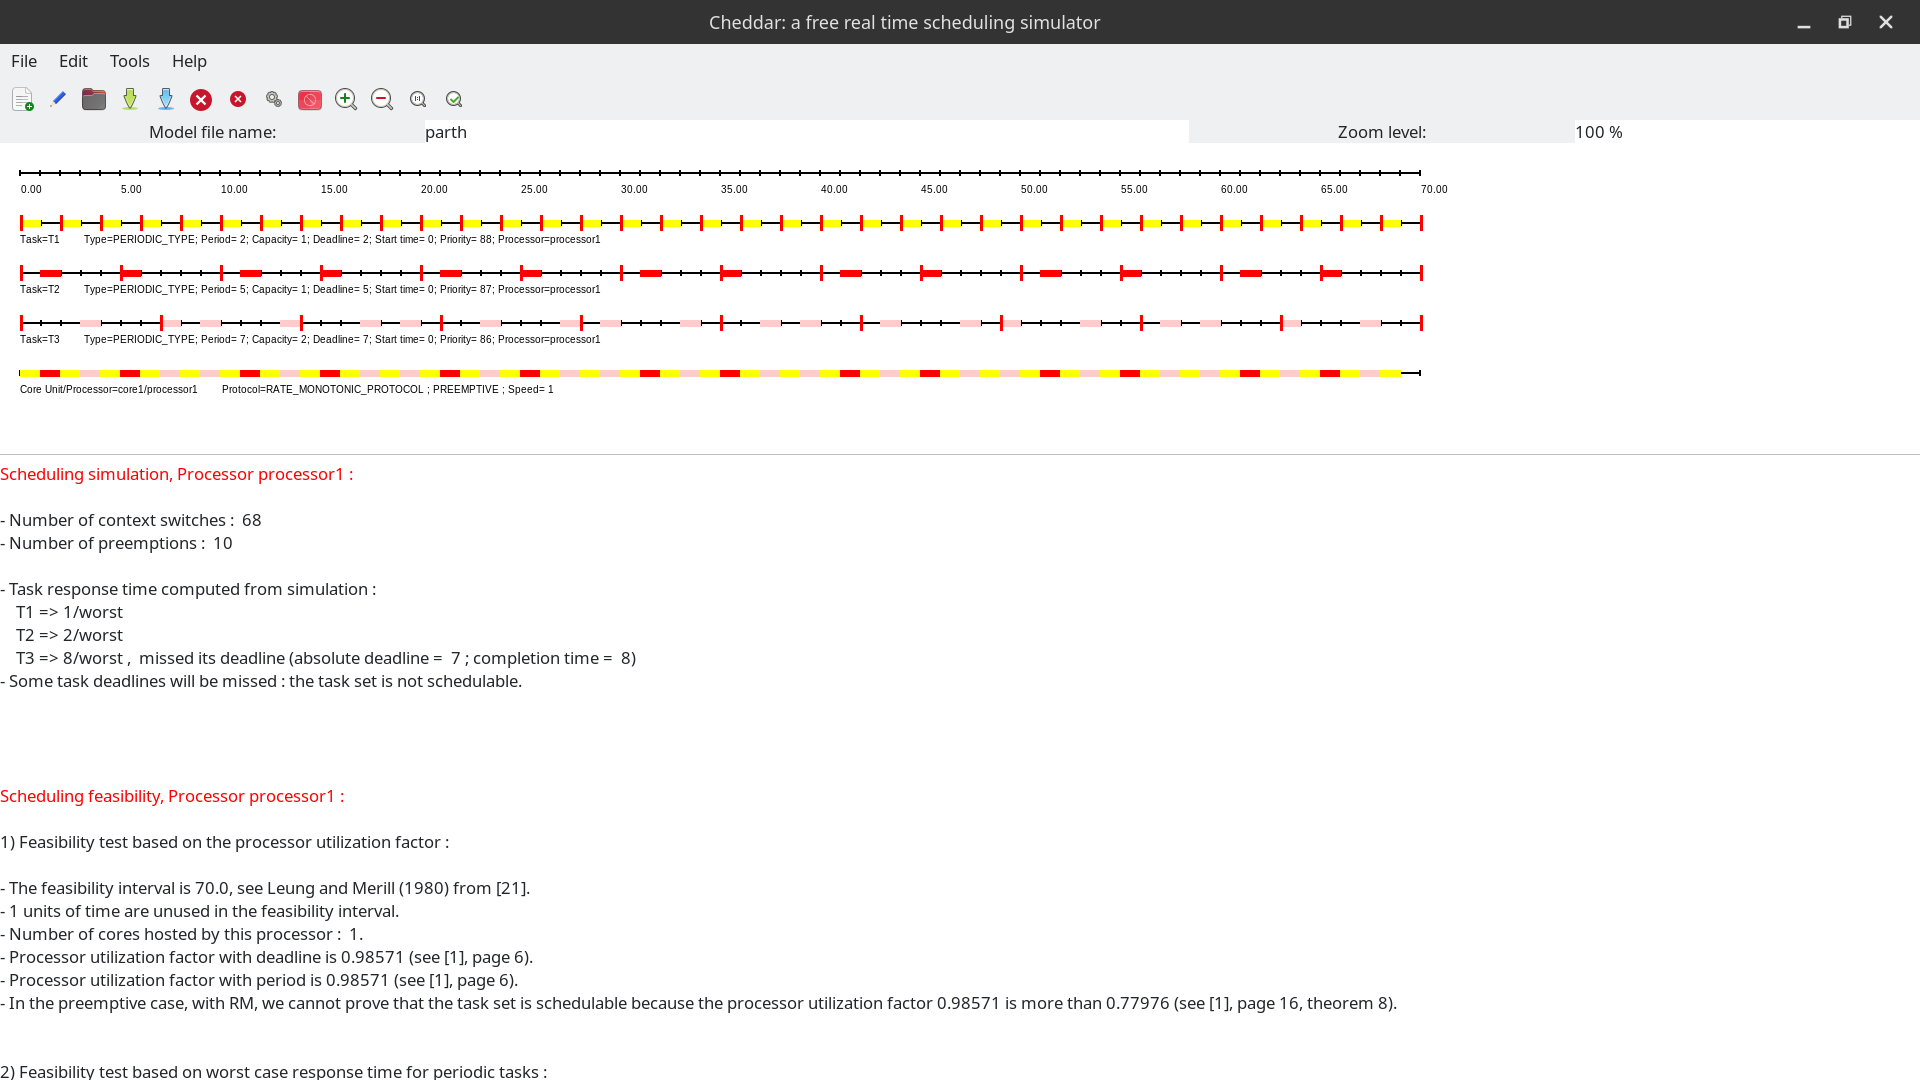
\includegraphics[scale=0.36]{figures/example1_rm.png}
							                  \caption{Example 1, RM analysis}
						                  \end{figure}
						            \item \textbf{Code Output:}\\
						                  \begin{verbatim}
****************
Example 1
C: 1 1 2
T: 2 5 7
D: 2 5 7

Task 0, WCET=1, Period=2, Utility Sum = 0.500000
Task 1, WCET=1, Period=5, Utility Sum = 0.700000
Task 2, WCET=2, Period=7, Utility Sum = 0.985714

Total Utility Sum = 0.985714
LUB = 0.779763
RM LUB: Infeasible
Completion time feasibility: Infeasible
Scheduling point feasibility: Infeasible
										\end{verbatim}
						            \item \textbf{Conclusion:}\\
						                  We found that the Least Upper Bound (LUB) value is 0.779763, both in our code and when we checked with the Cheddar software, so our findings match. However, the CPU usage we calculated is quite high, at about 98.57\%, and this same high usage shows up in Cheddar as well when looking at task periods and deadlines.\\

						                  Because the LUB value is higher than the actual CPU usage RM\_LUB would fail in the test, and our checks for nessesarry and sufficient tests Completion time and Scheduling point tests are failing, that indicate that the tasks we set up can't all be completed within their deadlines according to Rate Monotonic (RM) scheduling rules. This means our tasks are set up in a way that causes some to miss their deadlines. Our results and the Cheddar output confirm that these tasks aren't feasible for the completion test and scheduling point feasibility.

						                  So these tasks are not Schedulable by RM policy.

					            \end{enumerate}
					            \addcontentsline{toc}{subsubsection}{Example 2}
					      \item \textbf{Example 2}
					            \begin{enumerate}
						            \item \textbf{Cheddar Output:}\\
						                  \begin{figure}[H]
							                  \centering
							                  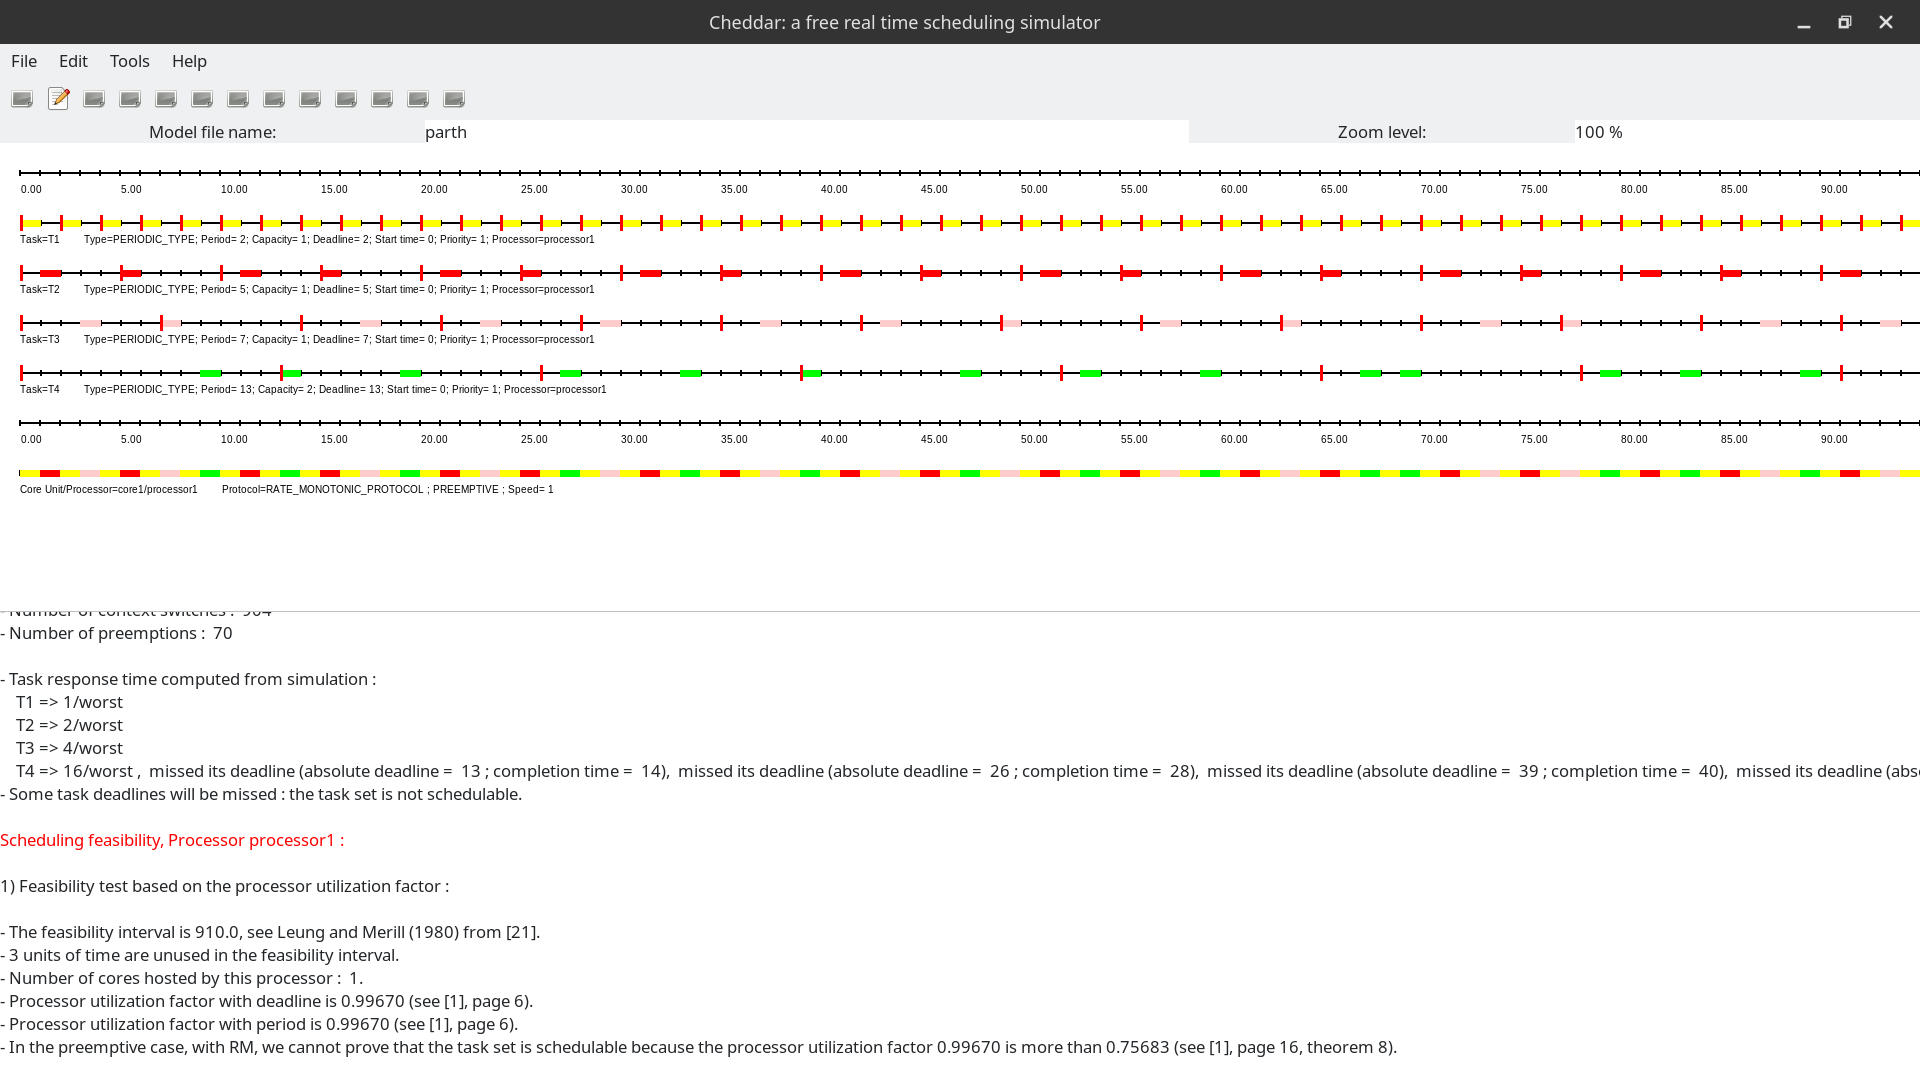
\includegraphics[scale=0.36]{figures/ex2_rm.png}
							                  \caption{Example 2, RM analysis}
						                  \end{figure}
						            \item \textbf{Code Output:}\\\\
						                  \begin{verbatim}
****************
Example 2
C: 1 1 1 2
T: 2 5 7 13
D: 2 5 7 13

Task 0, WCET=1, Period=2, Utility Sum = 0.500000
Task 1, WCET=1, Period=5, Utility Sum = 0.700000
Task 2, WCET=1, Period=7, Utility Sum = 0.842857
Task 3, WCET=2, Period=13, Utility Sum = 0.996703

Total Utility Sum = 0.996703
LUB = 0.756828
RM LUB: Infeasible
Completion time feasibility: Infeasible
Scheduling point feasibility: Infeasible
										\end{verbatim}
						            \item \textbf{Conclusion:}\\
						                  We found that the Least Upper Bound (LUB) value is 0.756828, both in our code and when we checked with the Cheddar software, so our findings match. However, the CPU usage we calculated is quite high, at about 99.6703\%, and this same high usage shows up in Cheddar as well when looking at task periods and deadlines.\\

						                  Because the LUB value is higher than the actual CPU usage RM\_LUB would fail in the test, and our checks for nessesarry and sufficient tests Completion time and Scheduling point tests are failing, that indicate that the tasks we set up can't all be completed within their deadlines according to Rate Monotonic (RM) scheduling rules. This means our tasks are set up in a way that causes some to miss their deadlines. Our results and the Cheddar output confirm that these tasks aren't feasible for the completion test and scheduling point feasibility.\\

						                  So these tasks are not Schedulable by RM policy.


					            \end{enumerate}
					            \addcontentsline{toc}{subsubsection}{Example 3}
					      \item \textbf{Example 3}
					            \begin{enumerate}
						            \item \textbf{Cheddar Output:}\\
						                  \begin{figure}[H]
							                  \centering
							                  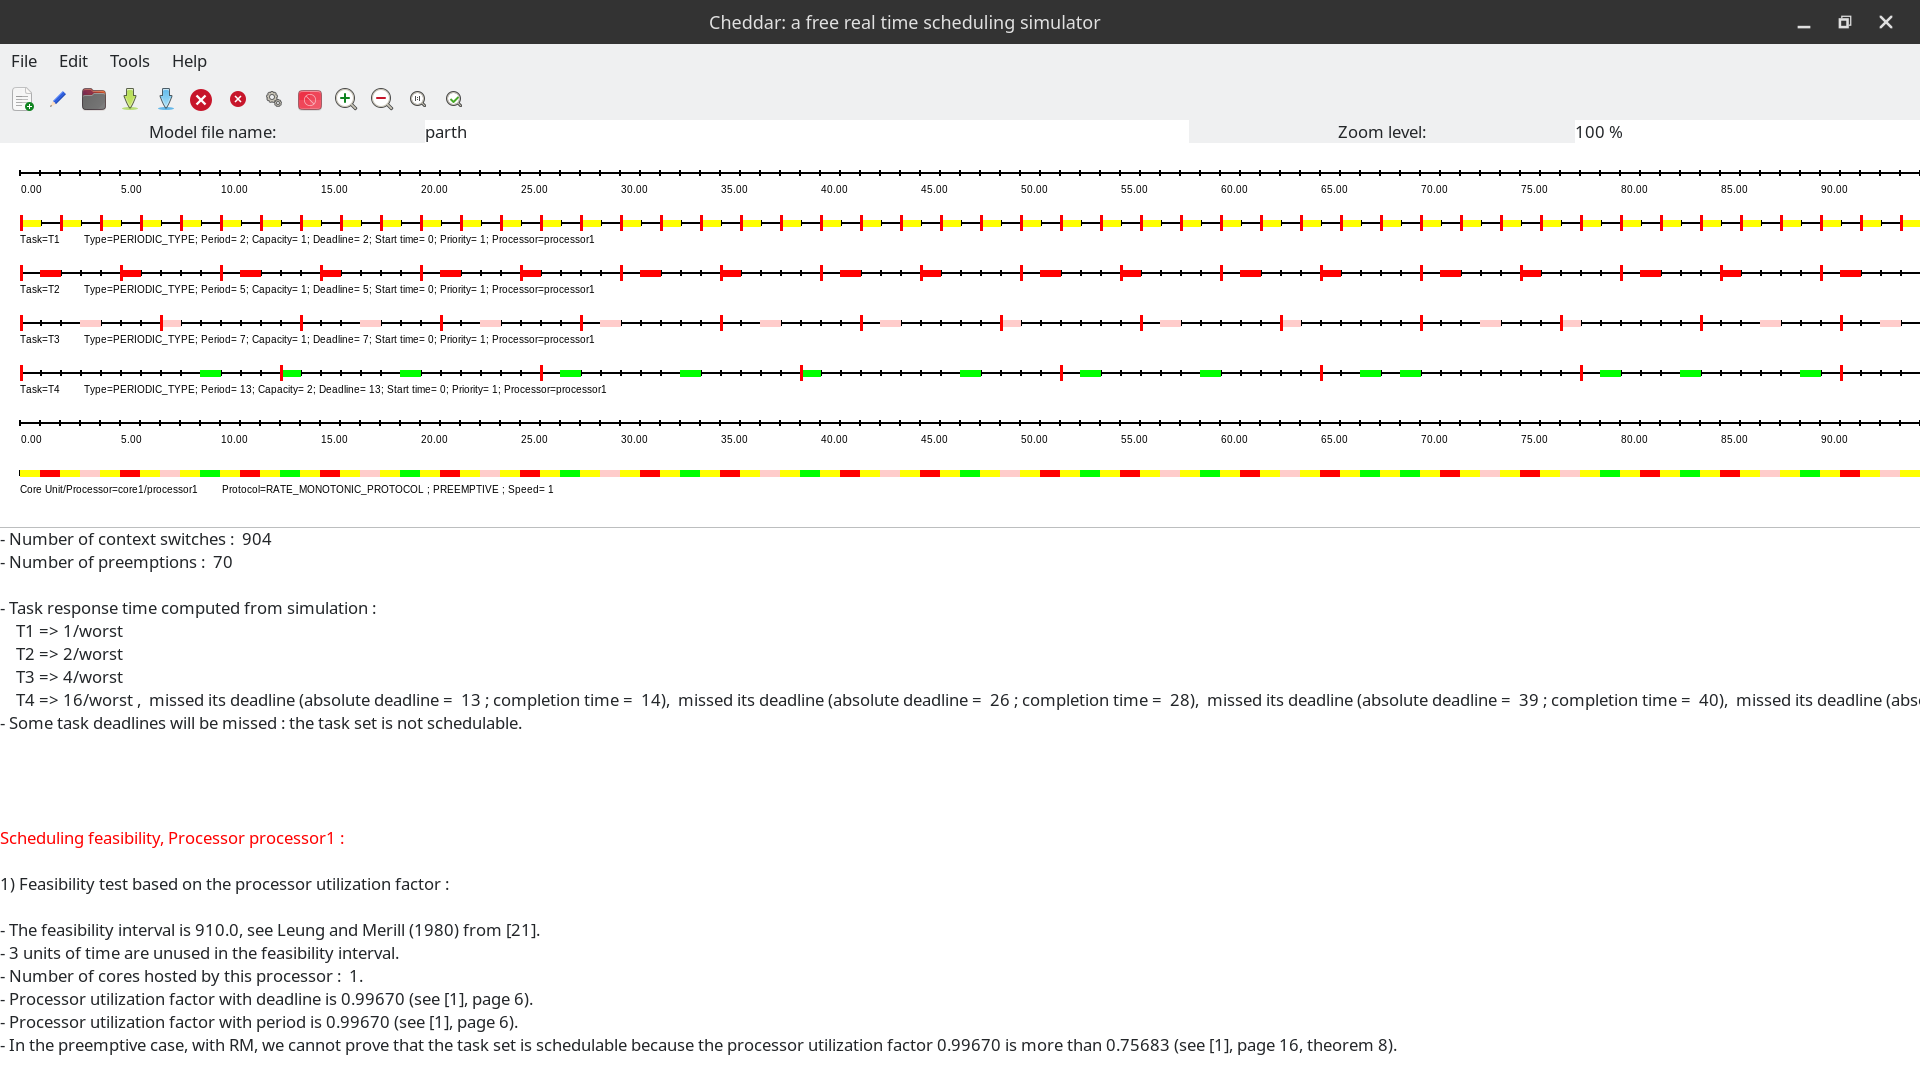
\includegraphics[scale=0.36]{figures/ex3_rm.png}
							                  \caption{Example 3, RM analysis}
						                  \end{figure}
						            \item \textbf{Code Output:}\\
						                  \begin{verbatim}
****************
Example 3
C: 1 2 3
T: 3 5 15
D: 3 5 15

Task 0, WCET=1, Period=3, Utility Sum = 0.333333
Task 1, WCET=2, Period=5, Utility Sum = 0.733333
Task 2, WCET=3, Period=15, Utility Sum = 0.933333

Total Utility Sum = 0.933333
LUB = 0.779763
RM LUB: Infeasible
Completion time feasibility: Feasible
Scheduling point feasibility: Feasible
										\end{verbatim}
						            \item \textbf{Conclusion:}\\
						                  We discovered that the Least Upper Bound (LUB) number is 0.779763, a figure that matches both in our own calculations and in the Cheddar software tests. However, we noticed that the CPU usage is really high, around 93.33\%, and this level of usage is also reflected in the Cheddar analysis when we look at the timing of tasks and their deadlines.\\

						                  Because the LUB value is higher than the actual CPU usage RM\_LUB would fail in the test, but all our checks for nessesarry and sufficient tests Completion time and Scheduling point feasibility shows that the tasks are feasible with RM schedule. This means we set up our tasks in a way that they can all get done within their set times without overloading the CPU. And we can confirm the results of no deadline miss in the cheddar.

						                  So these tasks are Schedulable by RM policy.

					            \end{enumerate}
					            \addcontentsline{toc}{subsubsection}{Example 4}
					      \item \textbf{Example 4}
					            \begin{enumerate}
						            \item \textbf{Cheddar Output:}\\
						                  \begin{figure}[H]
							                  \centering
							                  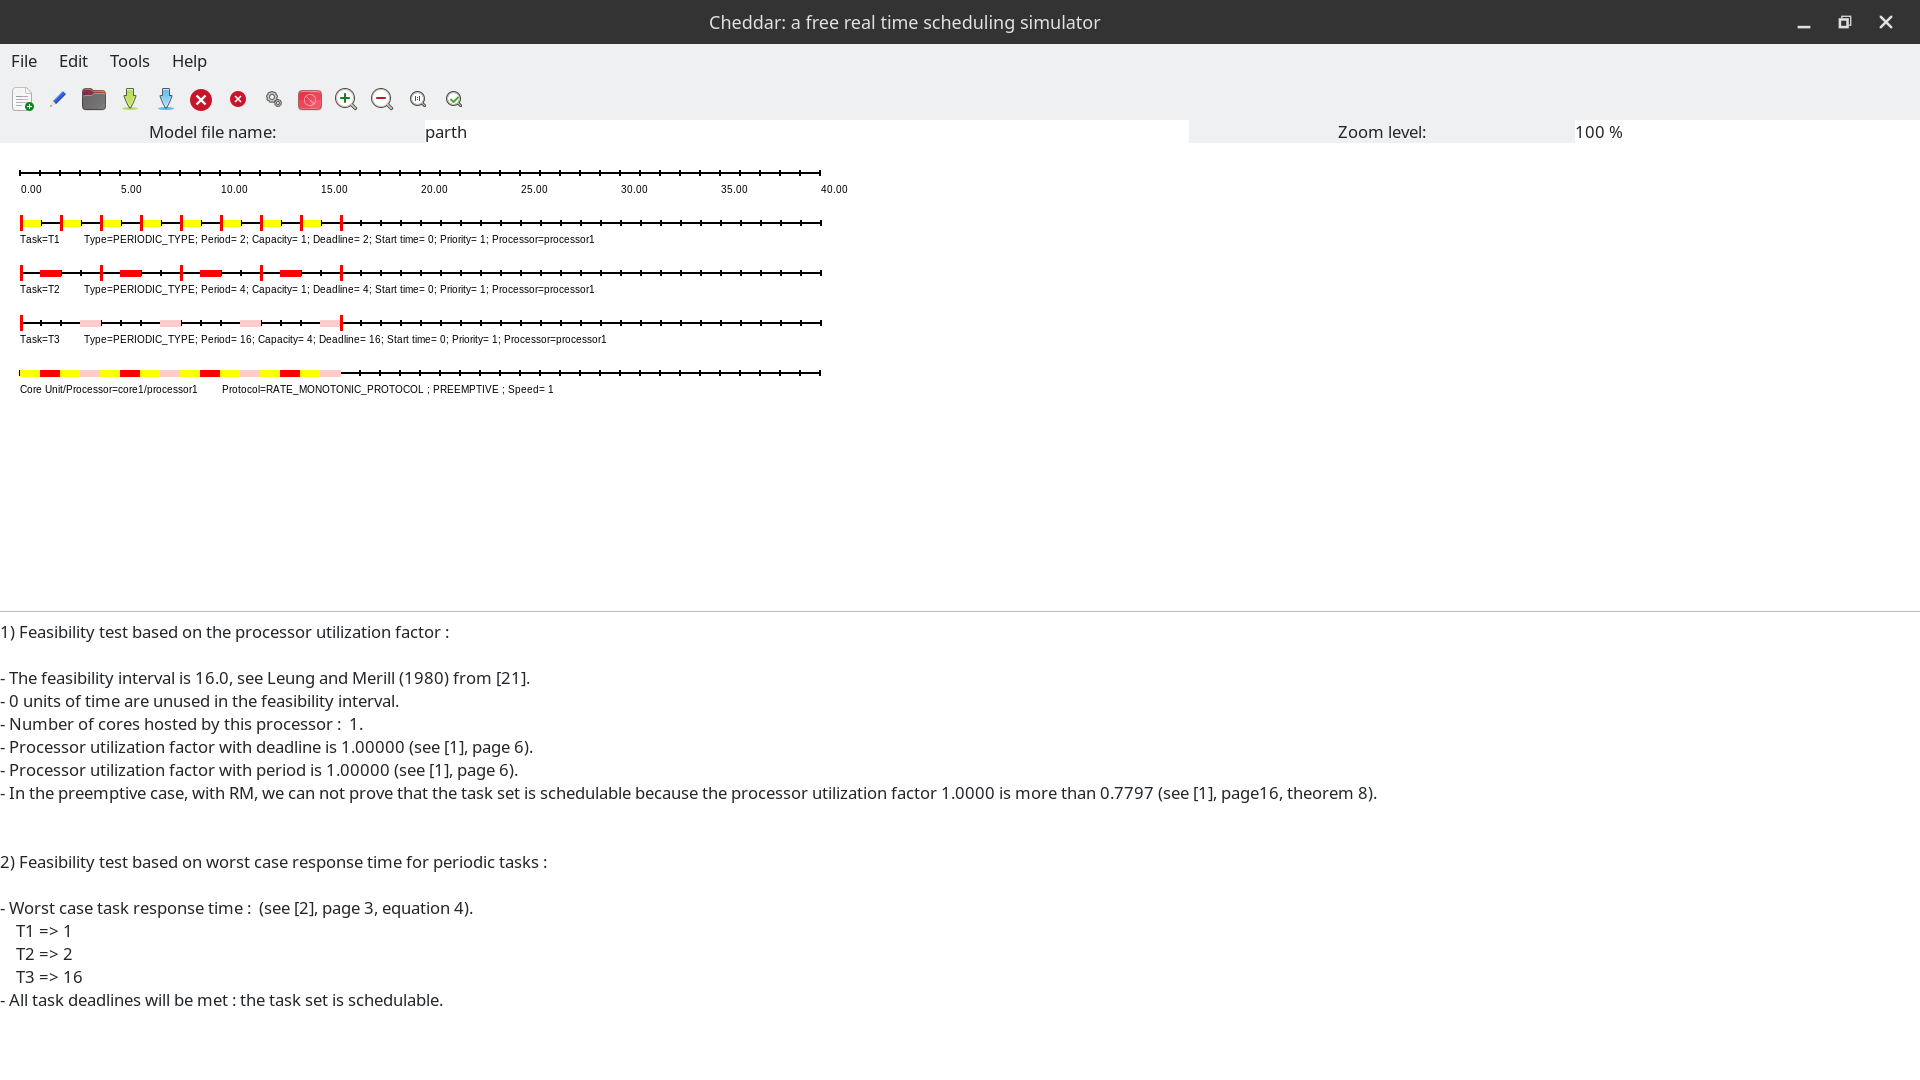
\includegraphics[scale=0.36]{figures/ex4_rm.png}
							                  \caption{Example 4, RM analysis}
						                  \end{figure}
						            \item \textbf{Code Output:}\\
						                  \begin{verbatim}
****************
Example 4
C: 1 1 4
T: 2 4 16
D: 2 4 16

Task 0, WCET=1, Period=2, Utility Sum = 0.500000
Task 1, WCET=1, Period=4, Utility Sum = 0.750000
Task 2, WCET=4, Period=16, Utility Sum = 1.000000

Total Utility Sum = 1.000000
LUB = 0.779763
RM LUB: Infeasible
Completion time feasibility: Feasible
Scheduling point feasibility: Feasible
										\end{verbatim}
						            \item \textbf{Conclusion:}\\
						                  The Least Upper Bound (LUB) number is 0.779763, a figure that matches both in our own calculations and in the Cheddar software tests. However, we noticed that the CPU usage is really high, around 100\%, and this level of usage is also reflected in the Cheddar analysis when we look at the timing of tasks and their deadlines.\\

						                  Because the LUB value is higher than the actual CPU usage RM\_LUB would fail in the test, but all our checks for nessesarry and sufficient tests Completion time and Scheduling point feasibility shows that the tasks are feasible with RM schedule. This means we set up our tasks in a way that they can all get done within their set times without overloading the CPU. And we can confirm the results of no deadline miss in the cheddar.\\

						                  So these tasks are Schedulable by RM policy.
					            \end{enumerate}
				      \end{enumerate}

				      \addcontentsline{toc}{subsection}{B}
				\item \Q Now, implement the remaining examples [5 more, 5-9] that we reviewed in class (found
				      here, and on Canvas) by modifying the example code to include the other examples.
				      Complete analysis for all three policies using Cheddar (RM, EDF, LLF) and by adding
				      EDF and LLF feasibility tests to the code, except for example 6, which should use RM
				      and DM. In cases where RM fails, but EDF or LLF succeeds, explain why. Cheddar
				      uses both service simulations over the LCM of the periods as well as feasibility analysis
				      based on the RM LUB and scheduling-point/completion-test algorithms, referred to as
				      “Worst Case Analysis”.

				      \A

				      \begin{enumerate}
					      \addcontentsline{toc}{subsubsection}{Example 5}
					      \item \textbf{Example 5}
					            \begin{enumerate}
						            \item \textbf{Cheddar Output:}\\

						                  \textbf{RM schedule}
						                  \begin{figure}[H]
							                  \centering
							                  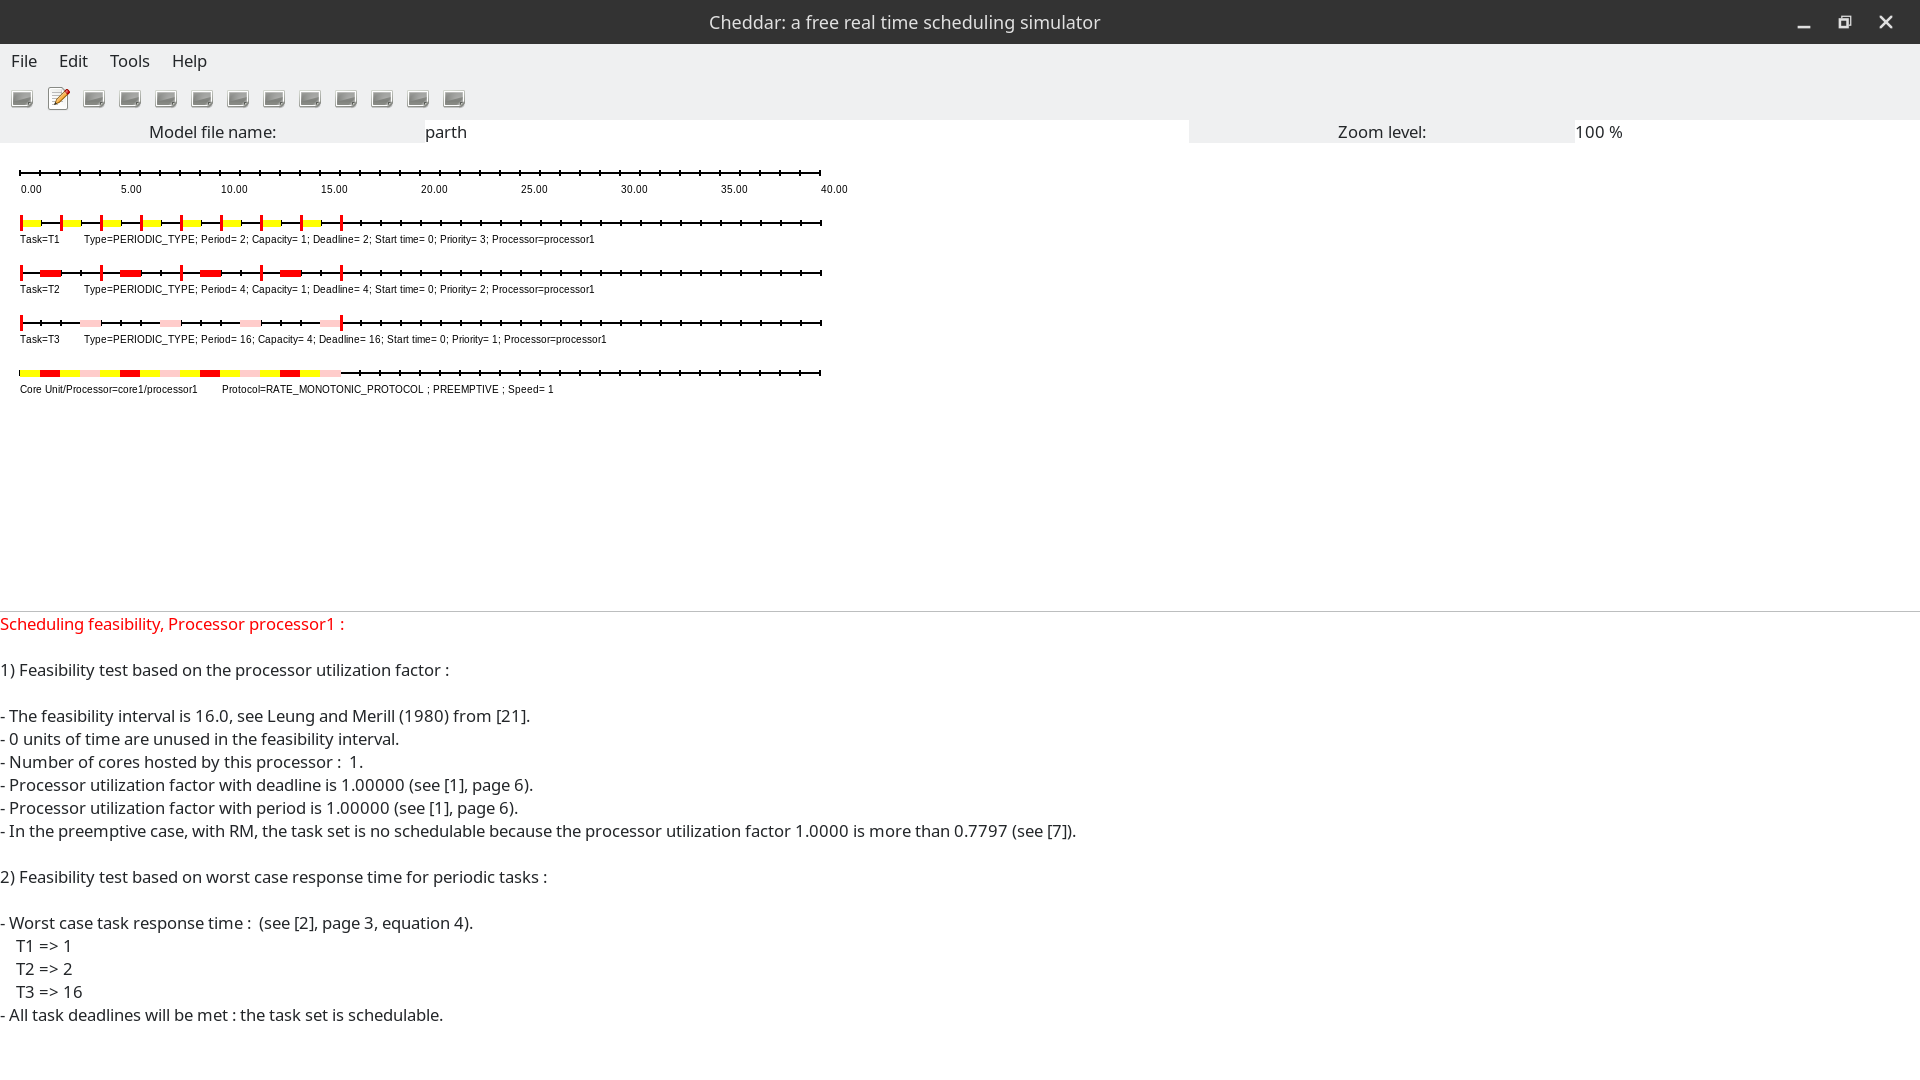
\includegraphics[scale=0.36]{figures/ex5_rm.png}
							                  \caption{Example 5, RM analysis}
						                  \end{figure}
						                  \textbf{EDF Schedule}
						                  \begin{figure}[H]
							                  \centering
							                  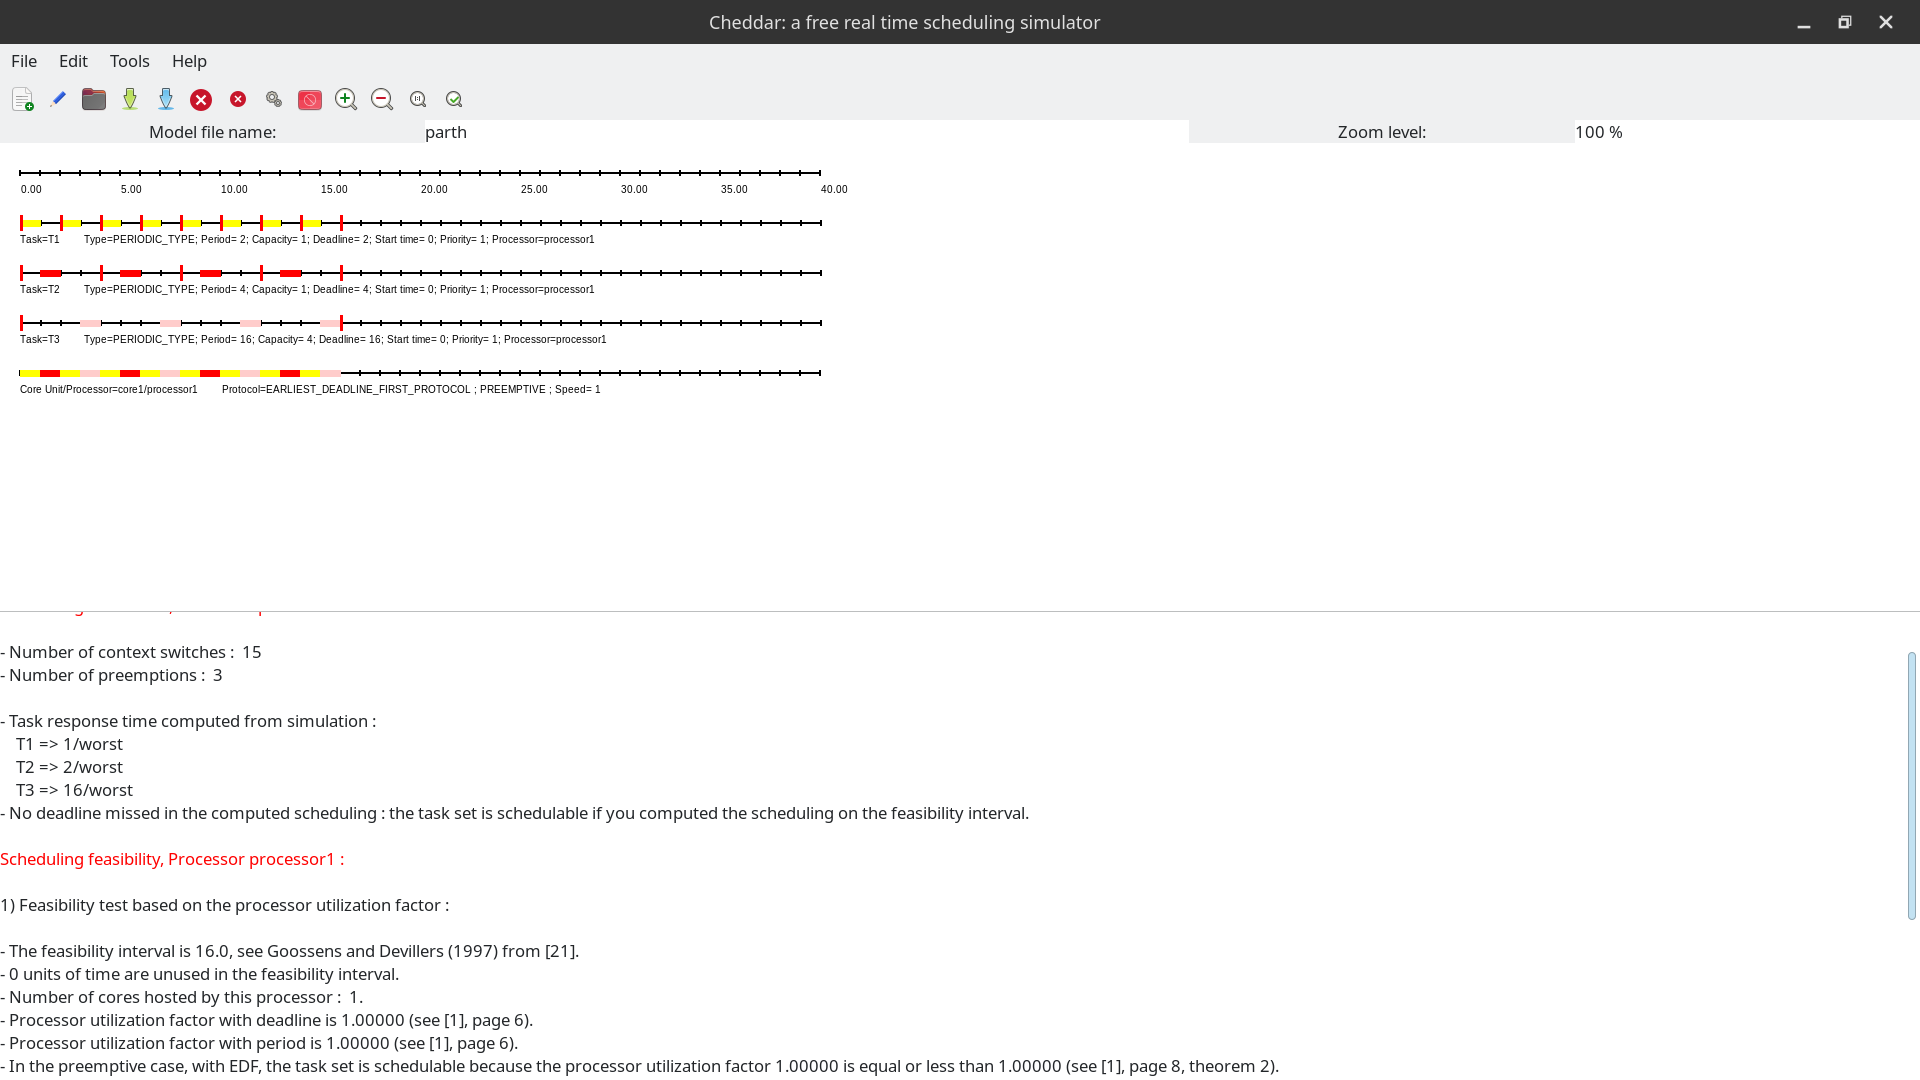
\includegraphics[scale=0.36]{figures/ex5_edf.png}
							                  \caption{Example 5, EDF analysis}
						                  \end{figure}
						                  \textbf{LLF Schedule}
						                  \begin{figure}[H]
							                  \centering
							                  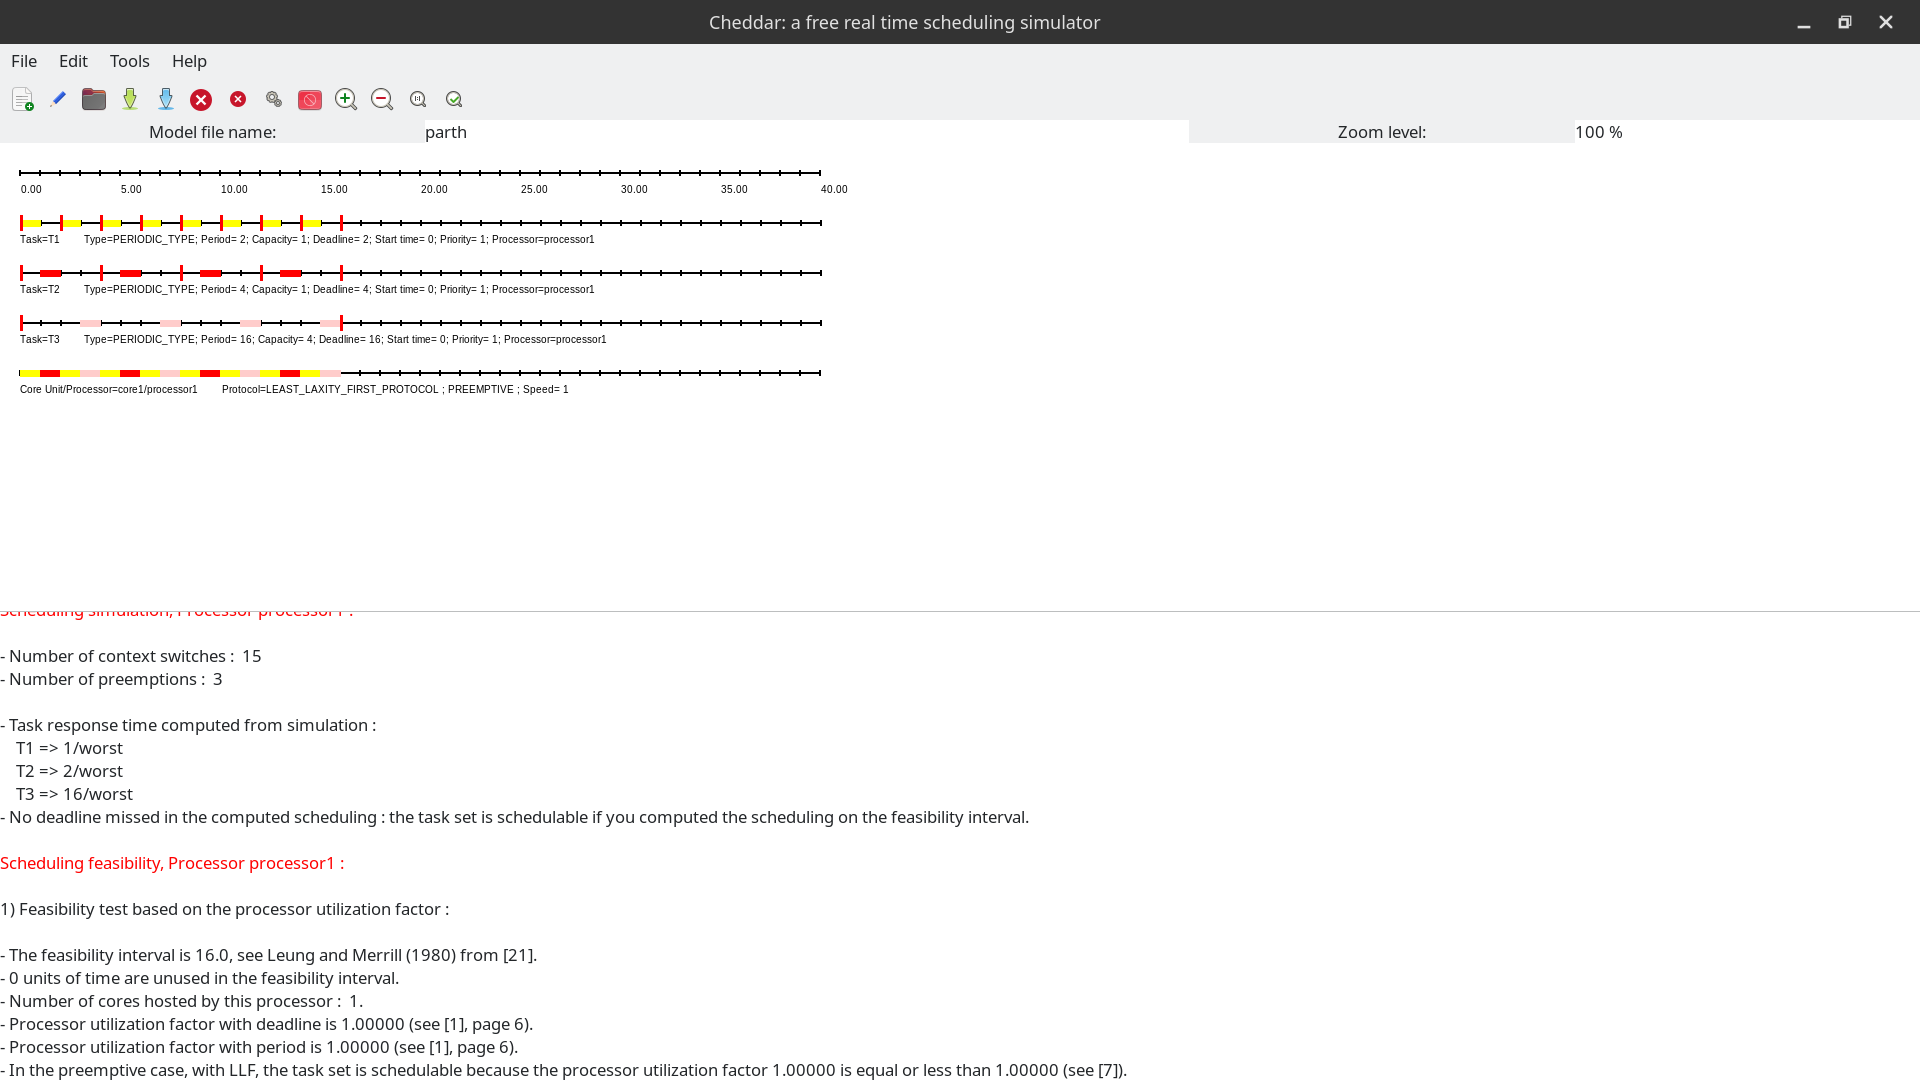
\includegraphics[scale=0.36]{figures/ex5_llf.png}
							                  \caption{Example 5, LLF analysis}
						                  \end{figure}


						            \item \textbf{Code Output:}\\
						                  \begin{verbatim}
****************
Example 5
C: 1 1 4
T: 2 4 16
D: 2 4 16

Task 0, WCET=1, Period=2, Utility Sum = 0.500000
Task 1, WCET=1, Period=4, Utility Sum = 0.750000
Task 2, WCET=4, Period=16, Utility Sum = 1.000000

Total Utility Sum = 1.000000
LUB = 0.779763
RM LUB: Infeasible
Completion time feasibility: Feasible
Scheduling point feasibility: Feasible

(Period)
Total utility in EDF: 1.000000 Which is less than 1.0
EDF: Feasible
Total utility in LLF: 1.000000 Which is less than 1.0
LLF: Feasible
										\end{verbatim}
						            \item \textbf{Conclusion:}\\
						                  The Least Upper Bound (LUB) number is 0.779763, a figure that matches both in our own calculations and in the Cheddar software tests. However, we noticed that the CPU usage is really high, around 100\%, and this level of usage is also reflected in the Cheddar analysis when we look at the timing of tasks and their deadlines.\\

						                  Because the LUB value is higher than the actual CPU usage RM\_LUB would fail in the test, but all our checks for nessesarry and sufficient tests Completion time and Scheduling point feasibility shows that the tasks are feasible with RM schedule. This means we set up our tasks in a way that they can all get done within their set times without overloading the CPU. And we can confirm the results of no deadline miss in the cheddar.\\

						                  The output of code for the EDF and LLF shows that these set of tasks are schedulable with EDF and LLF as the utilization is less than or equal to 100\% and we can see in the cheddar output that EDF and LLF are indeed feasible. Cheddar shows that in EDF or LLF, no deadlines are missed and therefor these set of tasks are feasible for EDF and LLF.\\

						                  So, these task are not schedulable by RM but can be schedulable by EDF or LLF Scheduling.
					            \end{enumerate}
					            \addcontentsline{toc}{subsubsection}{Example 6}
					      \item \textbf{Example 6}
					            \begin{enumerate}
						            \item \textbf{Cheddar Output:}\\
						                  \textbf{RM schedule}
						                  \begin{figure}[H]
							                  \centering
							                  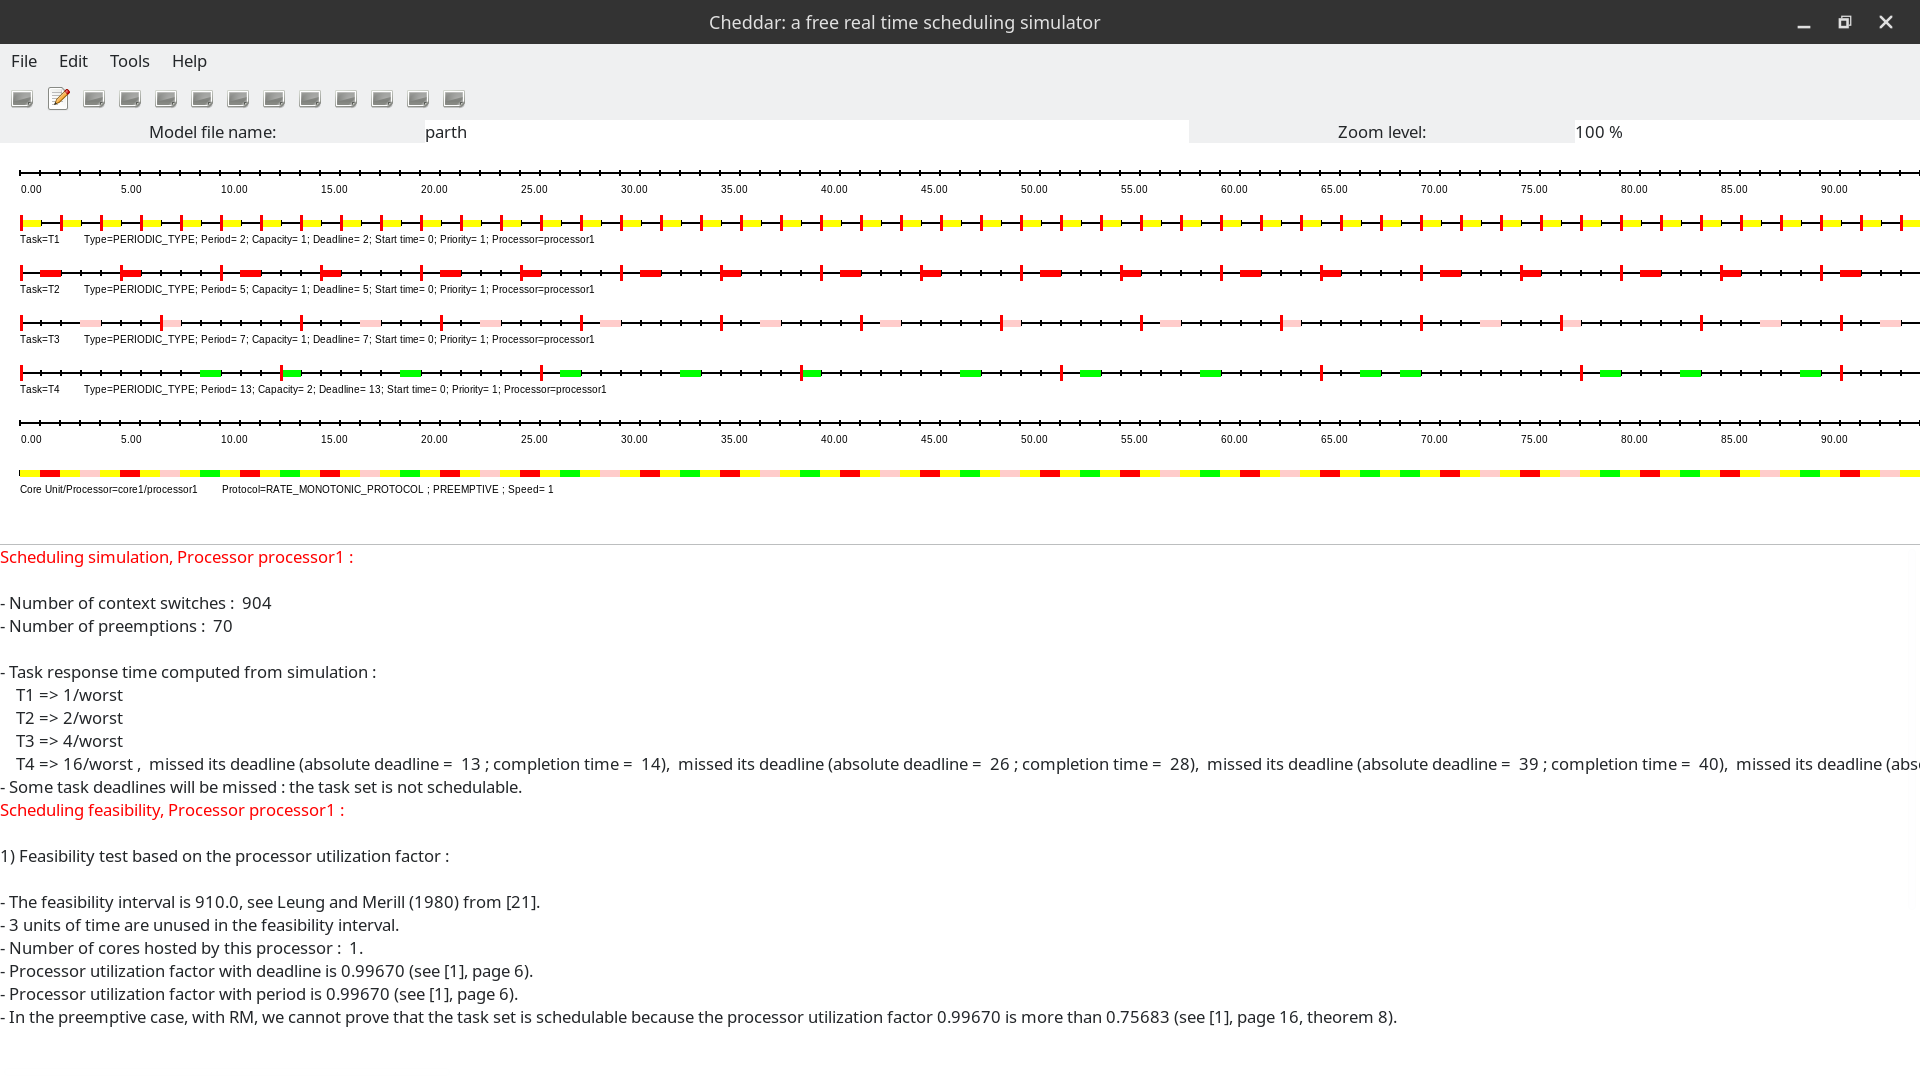
\includegraphics[scale=0.36]{figures/ex6_rm.png}
							                  \caption{Example 6, RM analysis}
						                  \end{figure}
						                  \textbf{EDF Schedule}
						                  \begin{figure}[H]
							                  \centering
							                  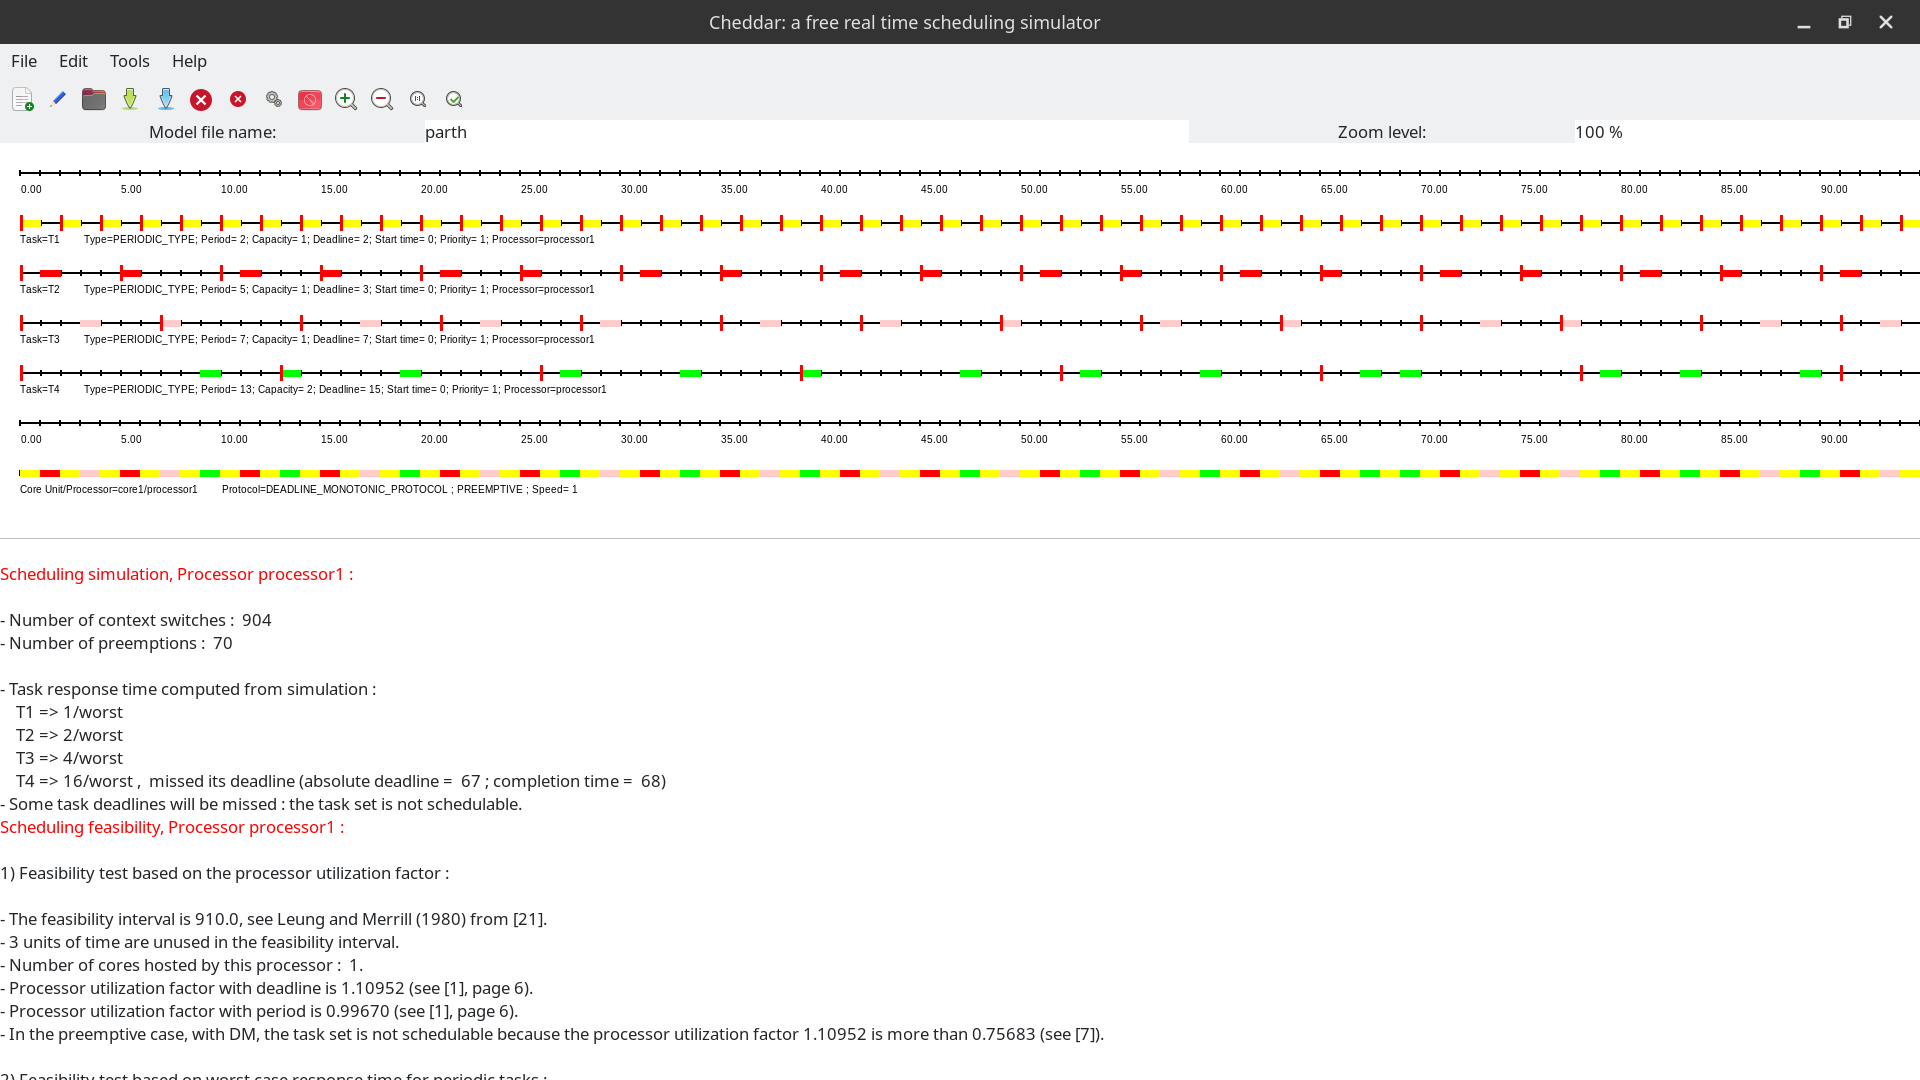
\includegraphics[scale=0.36]{figures/ex6_dm.png}
							                  \caption{Example 6, Deadline Monotonic analysis}
						                  \end{figure}
						            \item \textbf{Code Output:}\\
						                  \begin{verbatim}
****************
Example 6
C: 1 1 1 2
T: 2 5 7 13
D: 2 3 7 15

Task 0, WCET=1, Period=2, Utility Sum = 0.500000
Task 1, WCET=1, Period=5, Utility Sum = 0.700000
Task 2, WCET=1, Period=7, Utility Sum = 0.842857
Task 3, WCET=2, Period=13, Utility Sum = 0.996703

Total Utility Sum = 0.996703
LUB = 0.756828
RM LUB: Infeasible
Completion time feasibility: Infeasible
Scheduling point feasibility: Infeasible
Deadline monotonic: Infeasible

(Period)
Total utility in EDF: 0.996703 Which is less than 1.0
EDF on Period: Feasible
Total utility in LLF: 0.996703 Which is less than 1.0
LLF on Period: Feasible

(Deadline)
Total utility in EDF: 1.109524 Which is less than 1.0
EDF on Deadline: Infeasible
Total utility in LLF: 1.109524 Which is less than 1.0
LLF on Deadline: Infeasible
										\end{verbatim}
						            \item \textbf{Conclusion:}\\
						                  The Least Upper Bound (LUB) number is 0.756828, a figure that matches both in our own calculations and in the Cheddar software tests. However, we noticed that the CPU usage is really high, around 99.67\%, and this level of usage is also reflected in the Cheddar analysis when we look at the timing of tasks and their deadlines.\\

						                  Because the LUB value is higher than the actual CPU usage RM\_LUB would fail in the test, and our checks for nessesarry and sufficient tests Completion time and Scheduling point tests are failing, that indicate that the tasks we set up can't all be completed within their deadlines according to Rate Monotonic (RM) scheduling rules. This means our tasks are set up in a way that causes some to miss their deadlines. Our results and the Cheddar output confirm that these tasks aren't feasible for the completion test and scheduling point feasibility.\\

						                  Also Deadline monotonic feasibility test is failing in our case that can be confirmed by Cheddar's output for Deadline monotonic scheduling, we can see that in deadline monotonic scheduling cheddar shows one deadline is being missed. \\

						                  So, these task are not schedulable by Either RM or Deadline Monotonic Scheduling.

					            \end{enumerate}
					            \addcontentsline{toc}{subsubsection}{Example 7}
					      \item \textbf{Example 7}
					            \begin{enumerate}
						            \item \textbf{Cheddar Output:}\\
						                  \textbf{RM schedule}
						                  \begin{figure}[H]
							                  \centering
							                  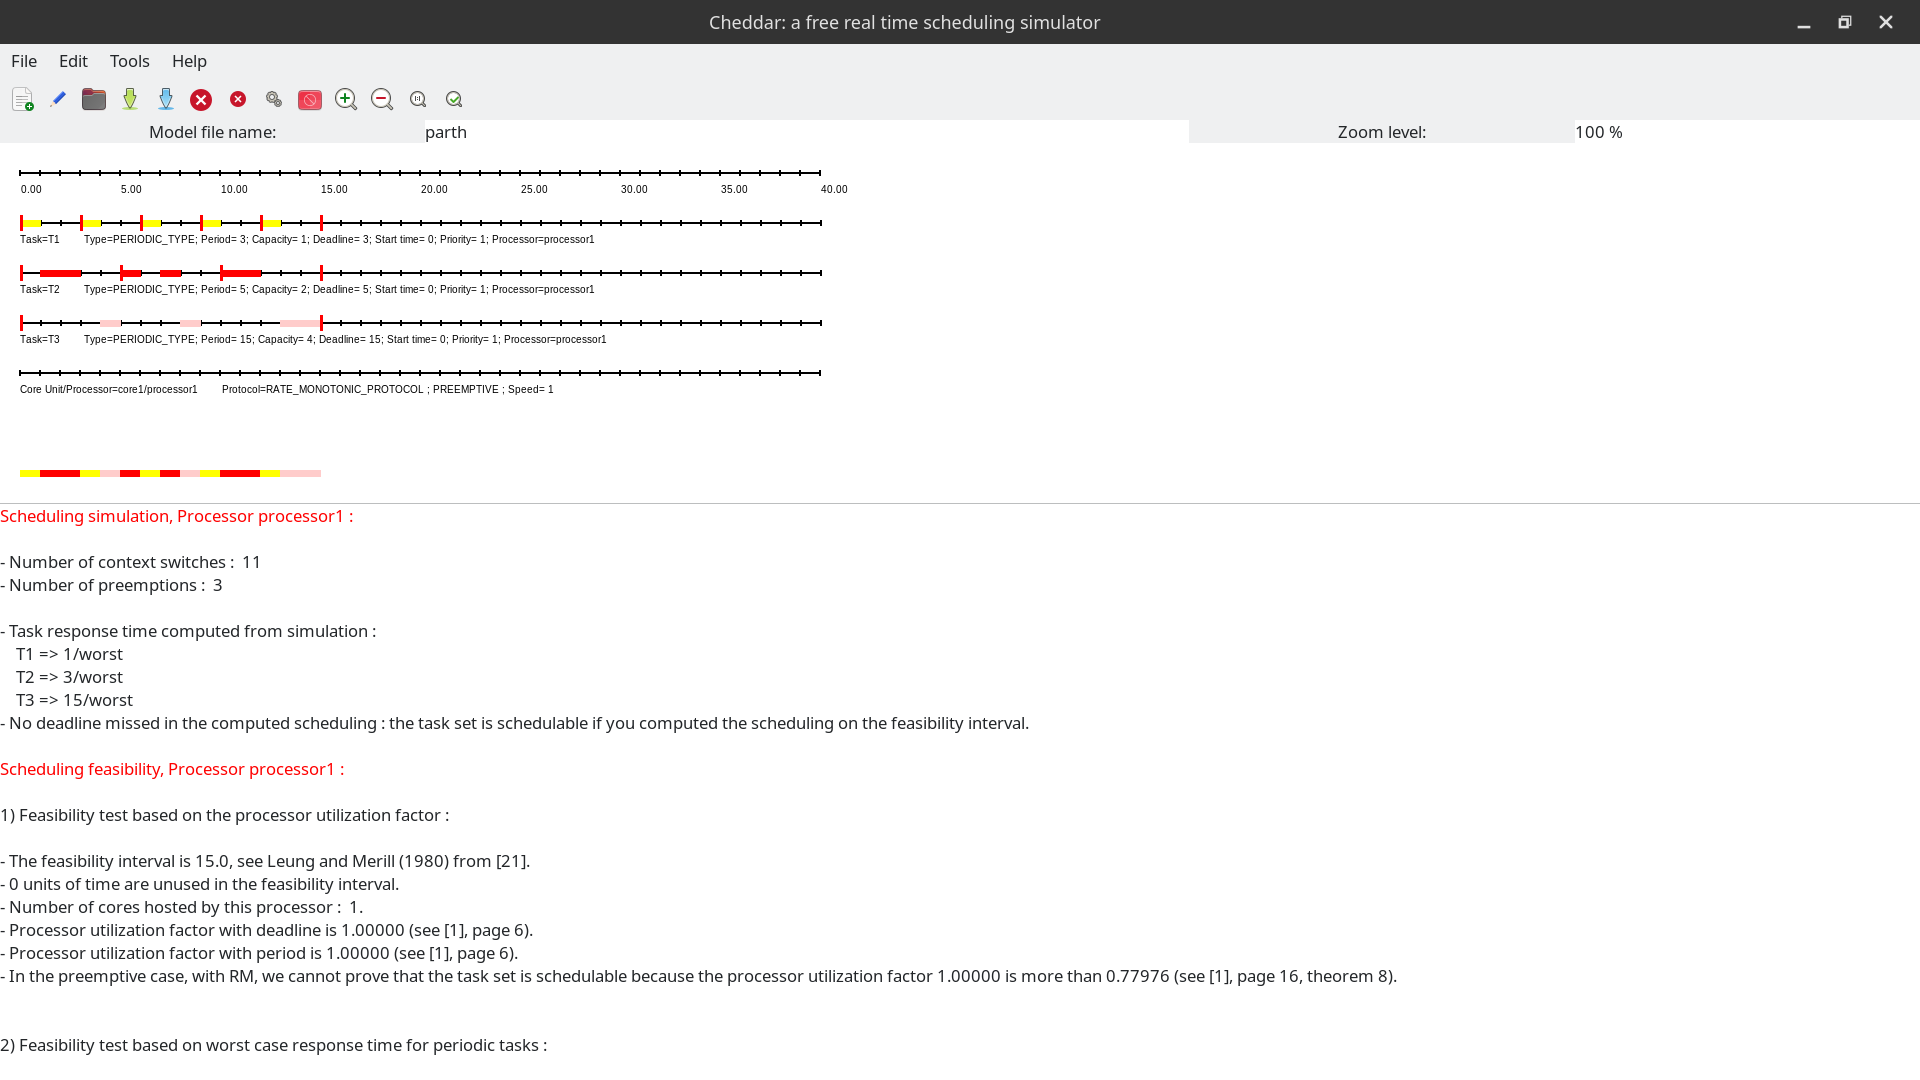
\includegraphics[scale=0.36]{figures/ex7_rm.png}
							                  \caption{Example 7, RM analysis}
						                  \end{figure}
						                  \textbf{EDF Schedule}
						                  \begin{figure}[H]
							                  \centering
							                  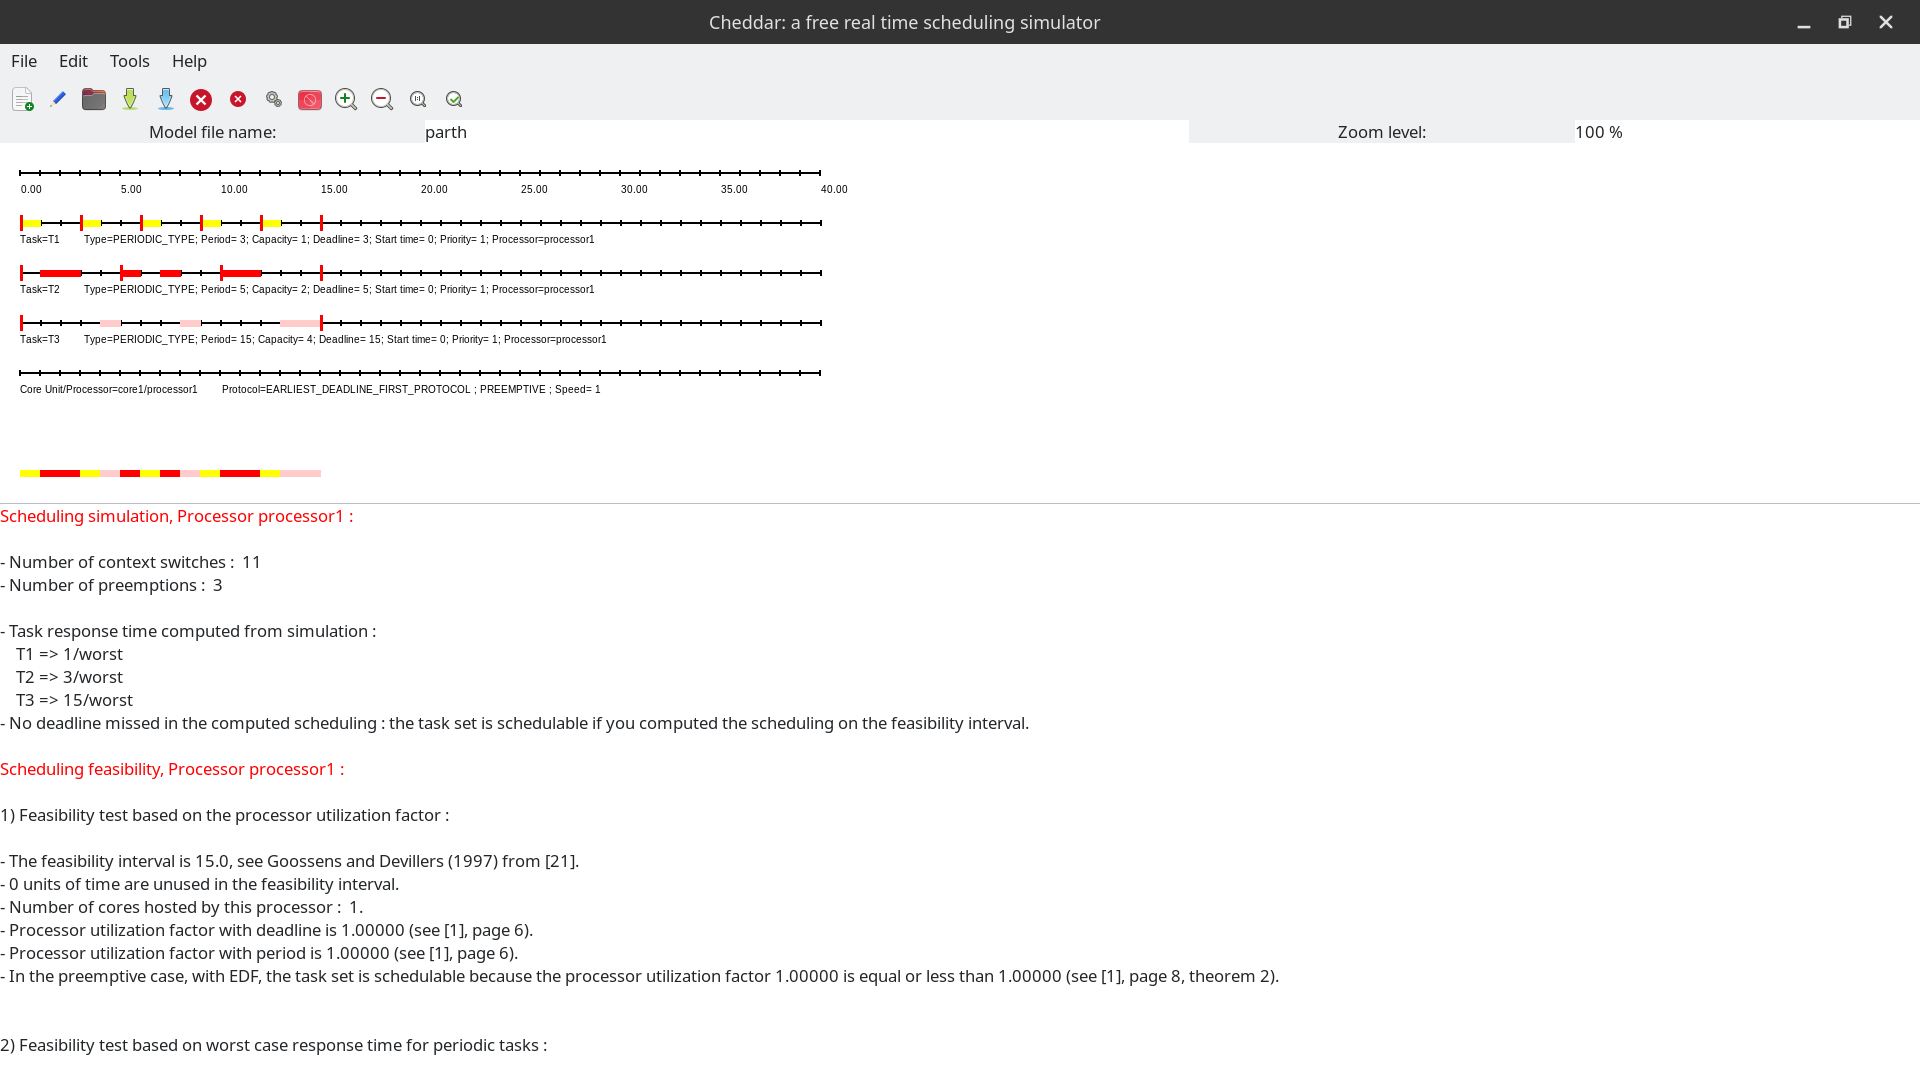
\includegraphics[scale=0.36]{figures/ex7_edf.png}
							                  \caption{Example 7, EDF analysis}
						                  \end{figure}
						                  \textbf{LLF Schedule}
						                  \begin{figure}[H]
							                  \centering
							                  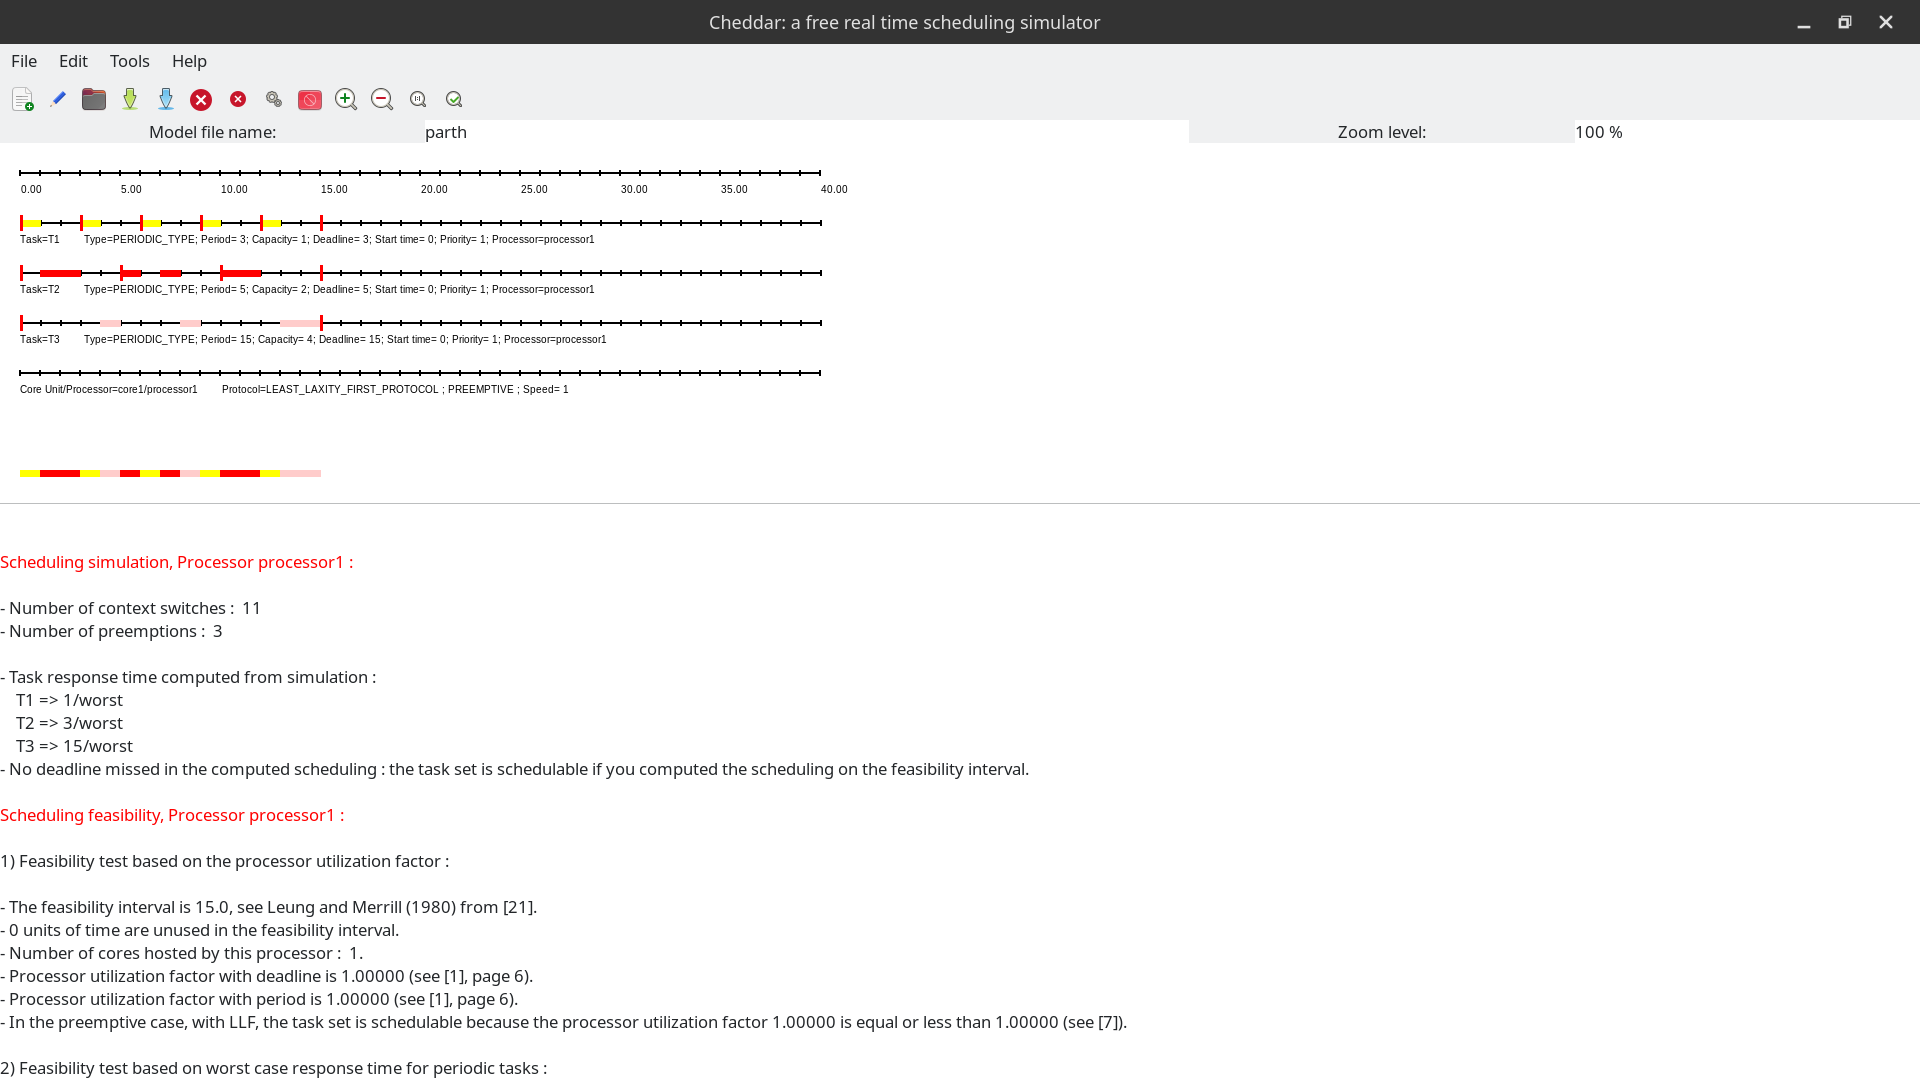
\includegraphics[scale=0.36]{figures/ex7_llf.png}
							                  \caption{Example 7, LLF analysis}
						                  \end{figure}
						            \item \textbf{Code Output:}\\
						                  \begin{verbatim}      
****************
Example 7
C: 1 2 4
T: 3 5 15
D: 3 5 15

Task 0, WCET=1, Period=3, Utility Sum = 0.333333
Task 1, WCET=2, Period=5, Utility Sum = 0.733333
Task 2, WCET=4, Period=15, Utility Sum = 1.000000

Total Utility Sum = 1.000000
LUB = 0.779763
RM LUB: Infeasible
Completion time feasibility: Feasible
Scheduling point feasibility: Feasible

(Period)
Total utility in EDF: 1.000000 Which is less than 1.0
EDF: Feasible
Total utility in LLF: 1.000000 Which is less than 1.0
LLF: Feasible
										\end{verbatim}
						            \item \textbf{Conclusion:}\\
						                  The Least Upper Bound (LUB) number is 0.779763, a figure that matches both in our own calculations and in the Cheddar software tests. However, we noticed that the CPU usage is really high, around 100.00\%, and this level of usage is also reflected in the Cheddar analysis when we look at the timing of tasks and their deadlines.\\

						                  Because the LUB value is higher than the actual CPU usage RM\_LUB would fail in the test, but all our checks for nessesarry and sufficient tests Completion time and Scheduling point feasibility shows that the tasks are feasible with RM schedule. This means we set up our tasks in a way that they can all get done within their set times without overloading the CPU. And we can confirm the results of no deadline miss in the cheddar.\\

						                  The output of code for the EDF and LLF shows that these set of tasks are schedulable with EDF and LLF as the utilization is less than or equal to 100\% and we can see in the cheddar output that EDF and LLF are indeed feasible. Cheddar shows that in EDF or LLF, no deadlines are missed and therefor these set of tasks are feasible for EDF and LLF.\\

						                  So, these task are schedulable by RM ,EDF or LLF Scheduling.

					            \end{enumerate}
					            \addcontentsline{toc}{subsubsection}{Example 8}
					      \item \textbf{Example 8}
					            \begin{enumerate}
						            \item \textbf{Cheddar Output:}\\
						                  \textbf{EDF Schedule}
						                  \begin{figure}[H]
							                  \centering
							                  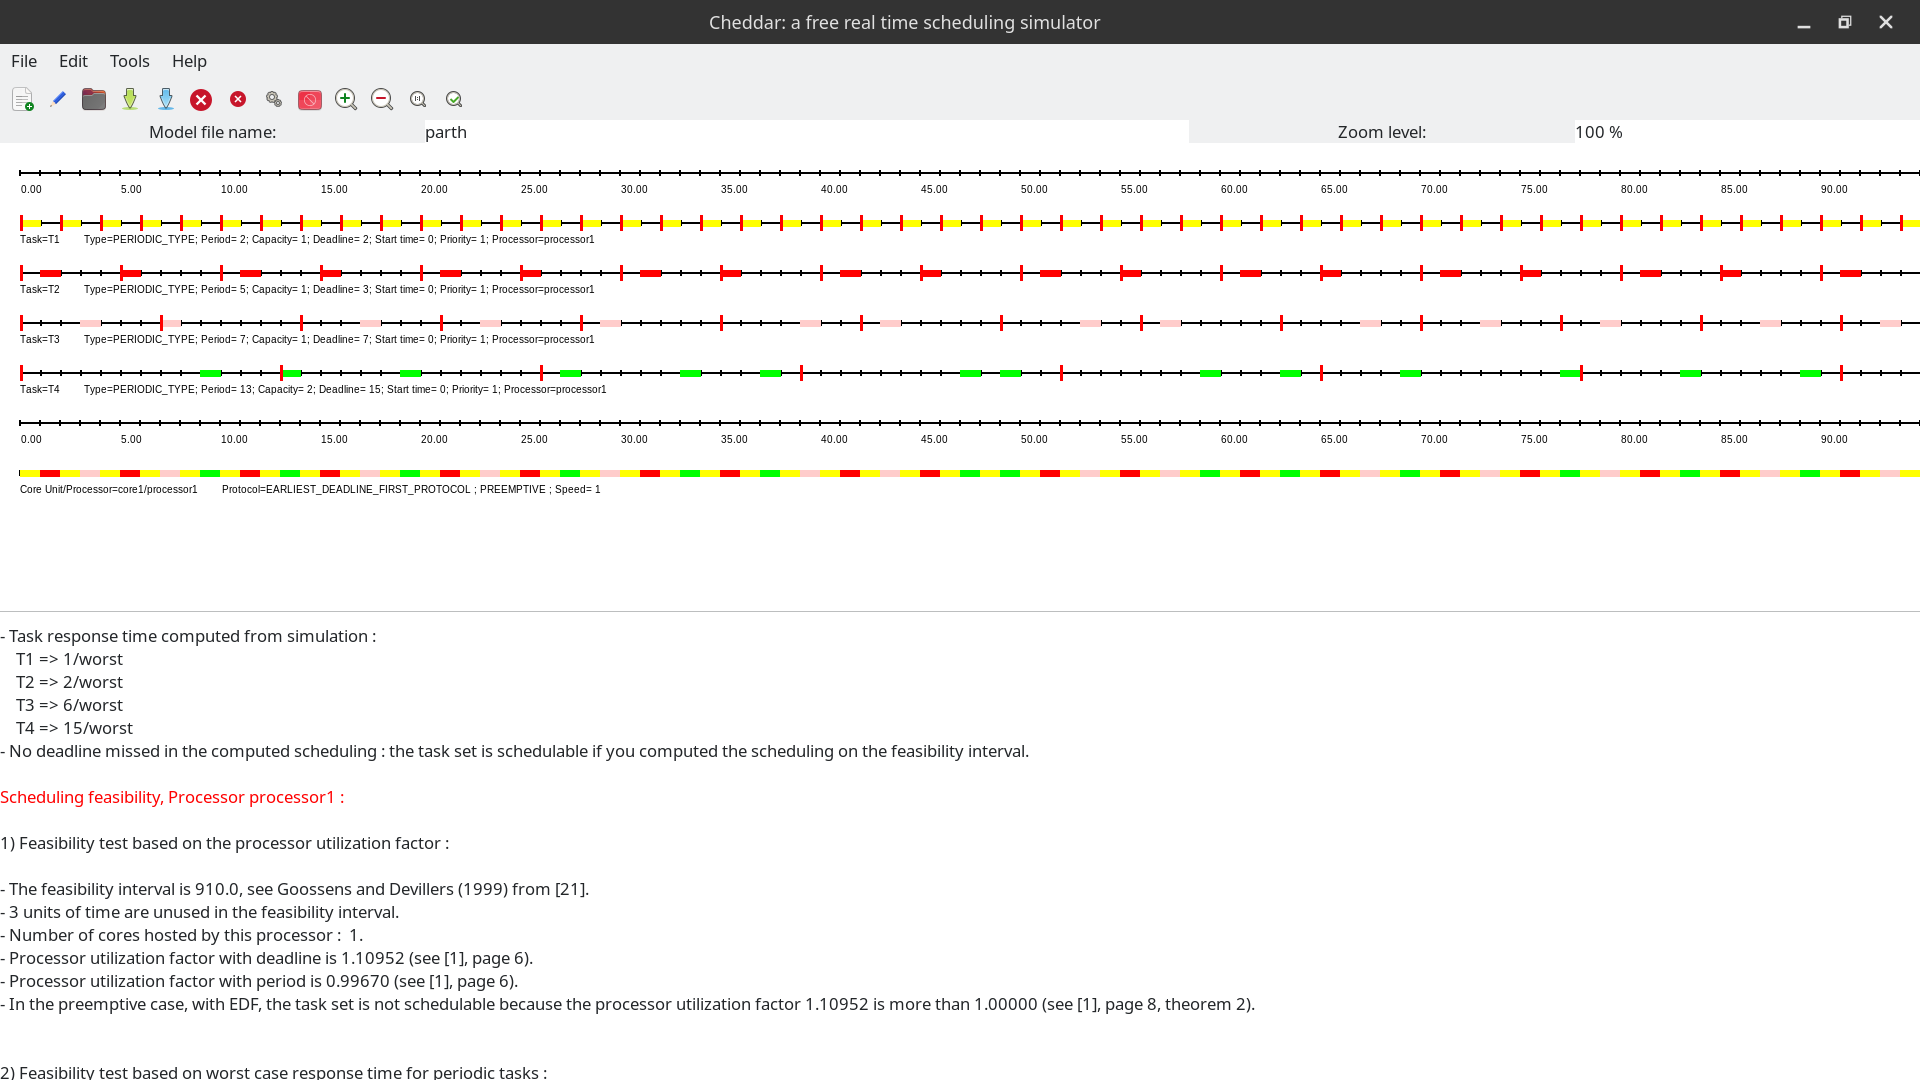
\includegraphics[scale=0.36]{figures/ex6_edf.png}
							                  \caption{Example 8, EDF analysis}
						                  \end{figure}
						                  \textbf{LLF Schedule}
						                  \begin{figure}[H]
							                  \centering
							                  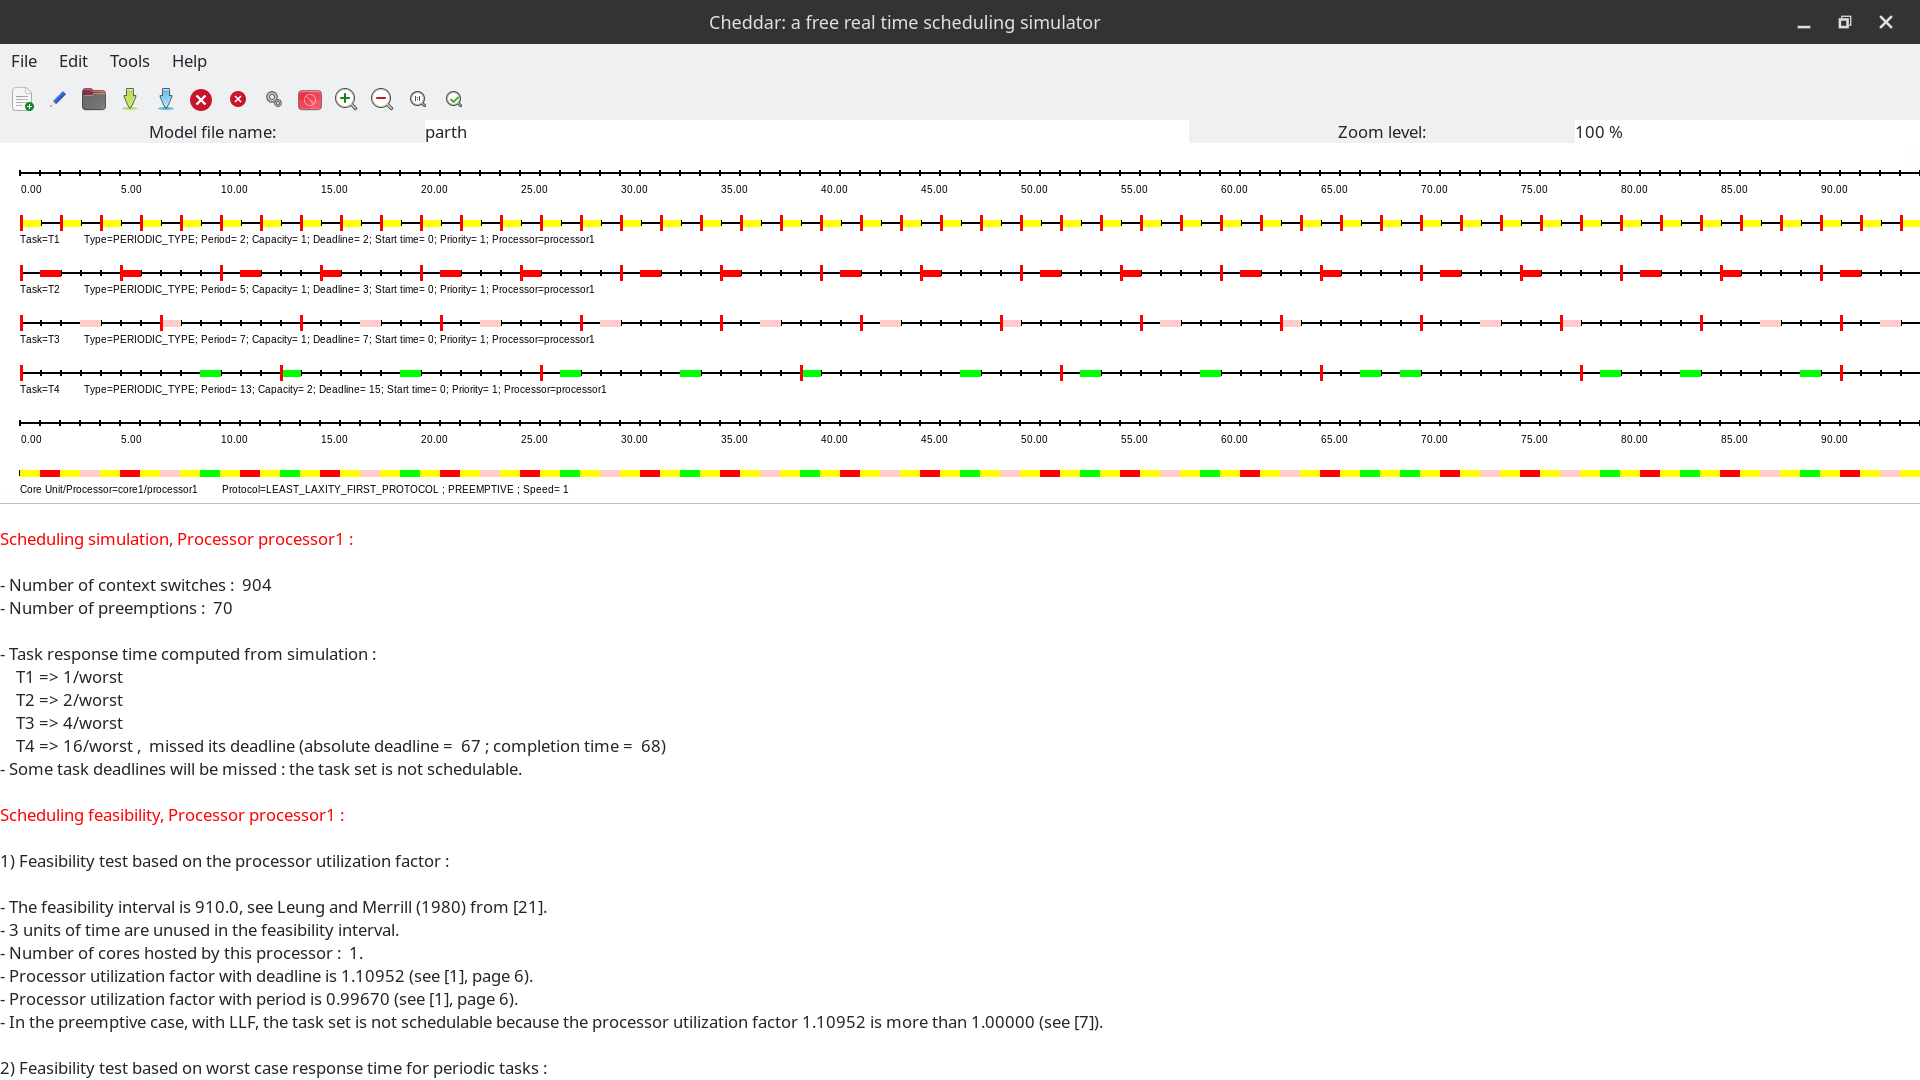
\includegraphics[scale=0.36]{figures/ex6_llf.png}
							                  \caption{Example 8, LLF analysis}
						                  \end{figure}
						            \item \textbf{Code Output:}\\
						                  \begin{verbatim}
****************
Example 8
C: 1 1 1 2
T: 2 5 7 13
D: 2 5 7 13

Task 0, WCET=1, Period=2, Utility Sum = 0.500000
Task 1, WCET=1, Period=5, Utility Sum = 0.700000
Task 2, WCET=1, Period=7, Utility Sum = 0.842857
Task 3, WCET=2, Period=13, Utility Sum = 0.996703

Total Utility Sum = 0.996703
LUB = 0.756828
RM LUB: Infeasible
Completion time feasibility: Infeasible
Scheduling point feasibility: Infeasible

(Period)
Total utility in EDF: 0.996703 Which is less than 1.0
EDF: Feasible
Total utility in LLF: 0.996703 Which is less than 1.0
LLF: Feasible
										\end{verbatim}
						            \item \textbf{Conclusion:}\\
						                  The Least Upper Bound (LUB) number is 0.756828, a figure that matches both in our own calculations and in the Cheddar software tests. However, we noticed that the CPU usage is really high, around 99.67\%, and this level of usage is also reflected in the Cheddar analysis when we look at the timing of tasks and their deadlines.\\

						                  Because the LUB value is higher than the actual CPU usage RM\_LUB would fail in the test, and our checks for nessesarry and sufficient tests Completion time and Scheduling point tests are failing, that indicate that the tasks we set up can't all be completed within their deadlines according to Rate Monotonic (RM) scheduling rules. This means our tasks are set up in a way that causes some to miss their deadlines. Our results and the Cheddar output confirm that these tasks aren't feasible for the completion test and scheduling point feasibility (RM\_Schedule).\\

						                  The output of code for the EDF and LLF shows that these set of tasks are schedulable with EDF and LLF as the utilization is less than or equal to 100\% and we can see in the cheddar output that EDF and LLF are indeed feasible. Cheddar shows that in EDF or LLF, no deadlines are missed and therefor these set of tasks are feasible for EDF and LLF.\\

						                  So, these task are not schedulable by RM but can be schedulable by EDF or LLF Scheduling.
					            \end{enumerate}
					            \addcontentsline{toc}{subsubsection}{Example 9}
					      \item \textbf{Example 9}
					            \begin{enumerate}
						            \item \textbf{Cheddar Output:}\\
						                  \textbf{RM schedule}
						                  \begin{figure}[H]
							                  \centering
							                  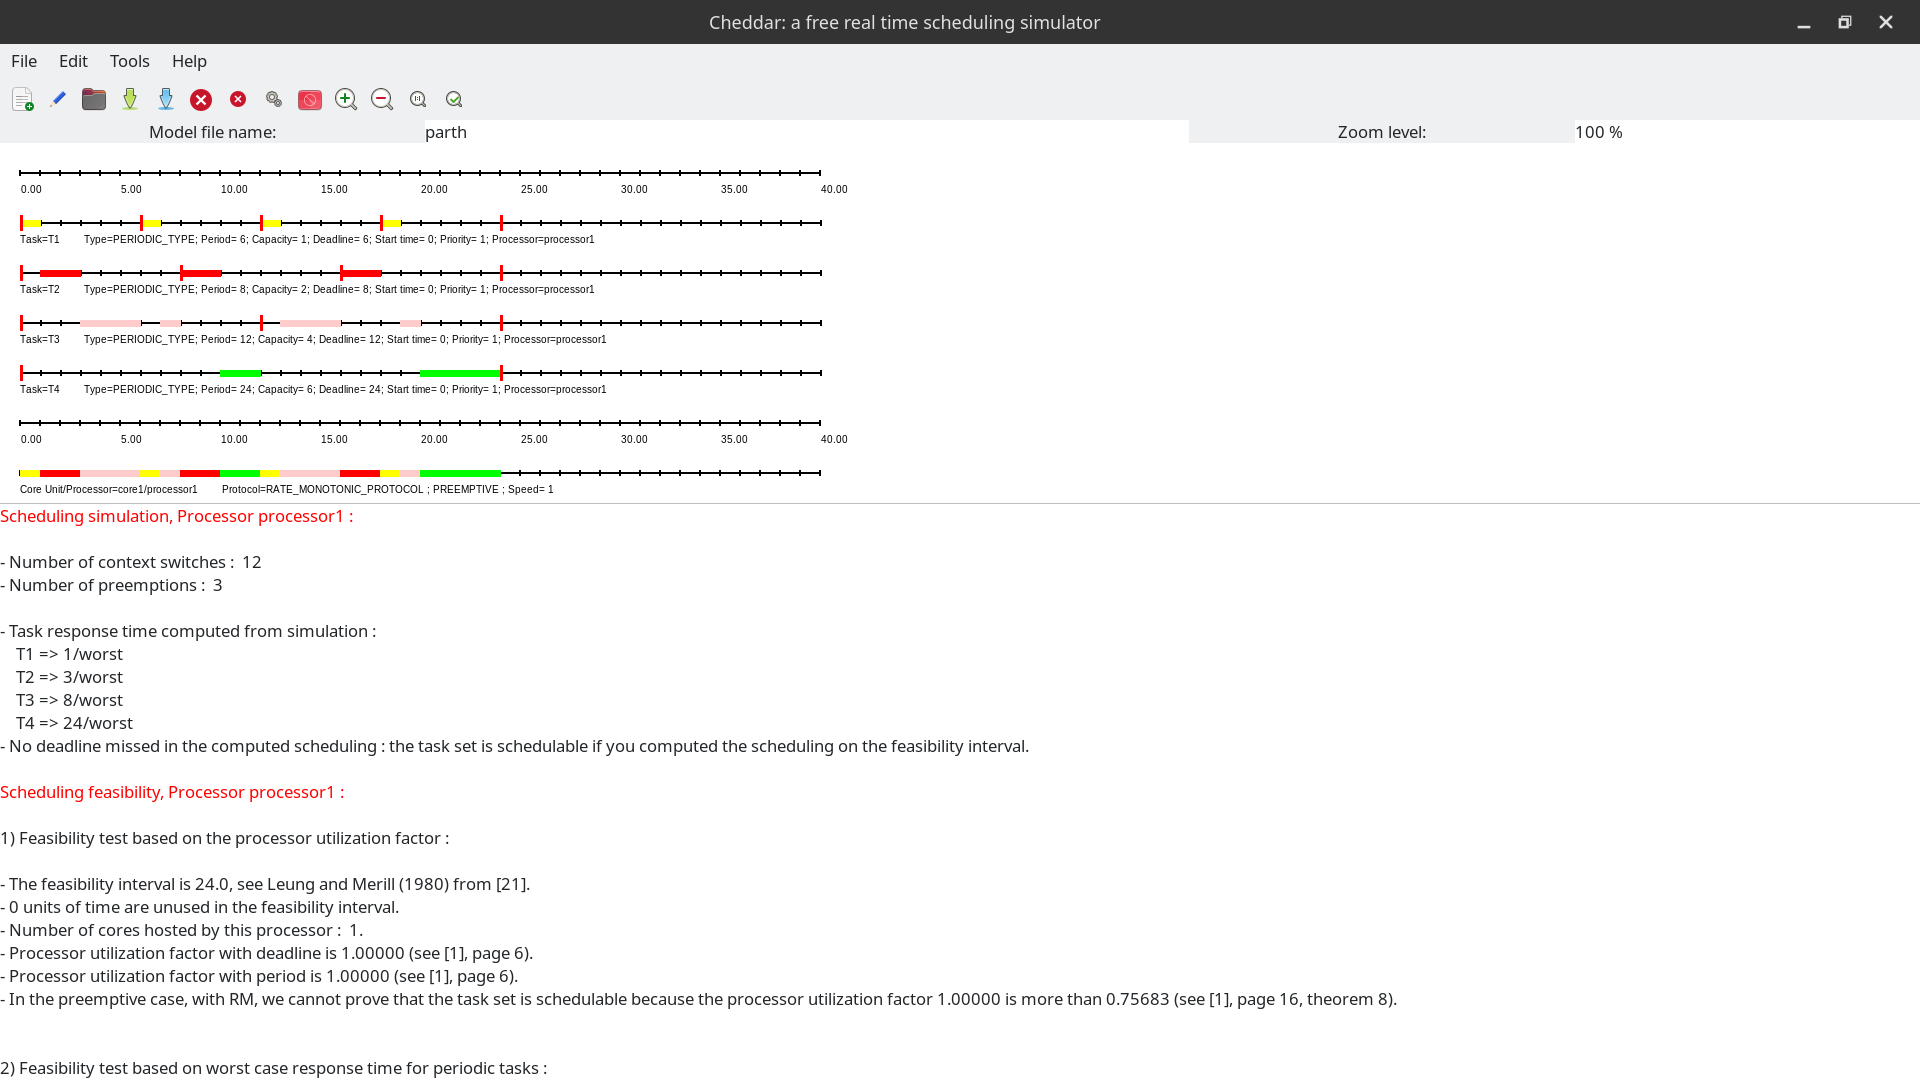
\includegraphics[scale=0.36]{figures/ex9_rm.png}
							                  \caption{Example 9, RM analysis}
						                  \end{figure}
						                  \textbf{EDF Schedule}
						                  \begin{figure}[H]
							                  \centering
							                  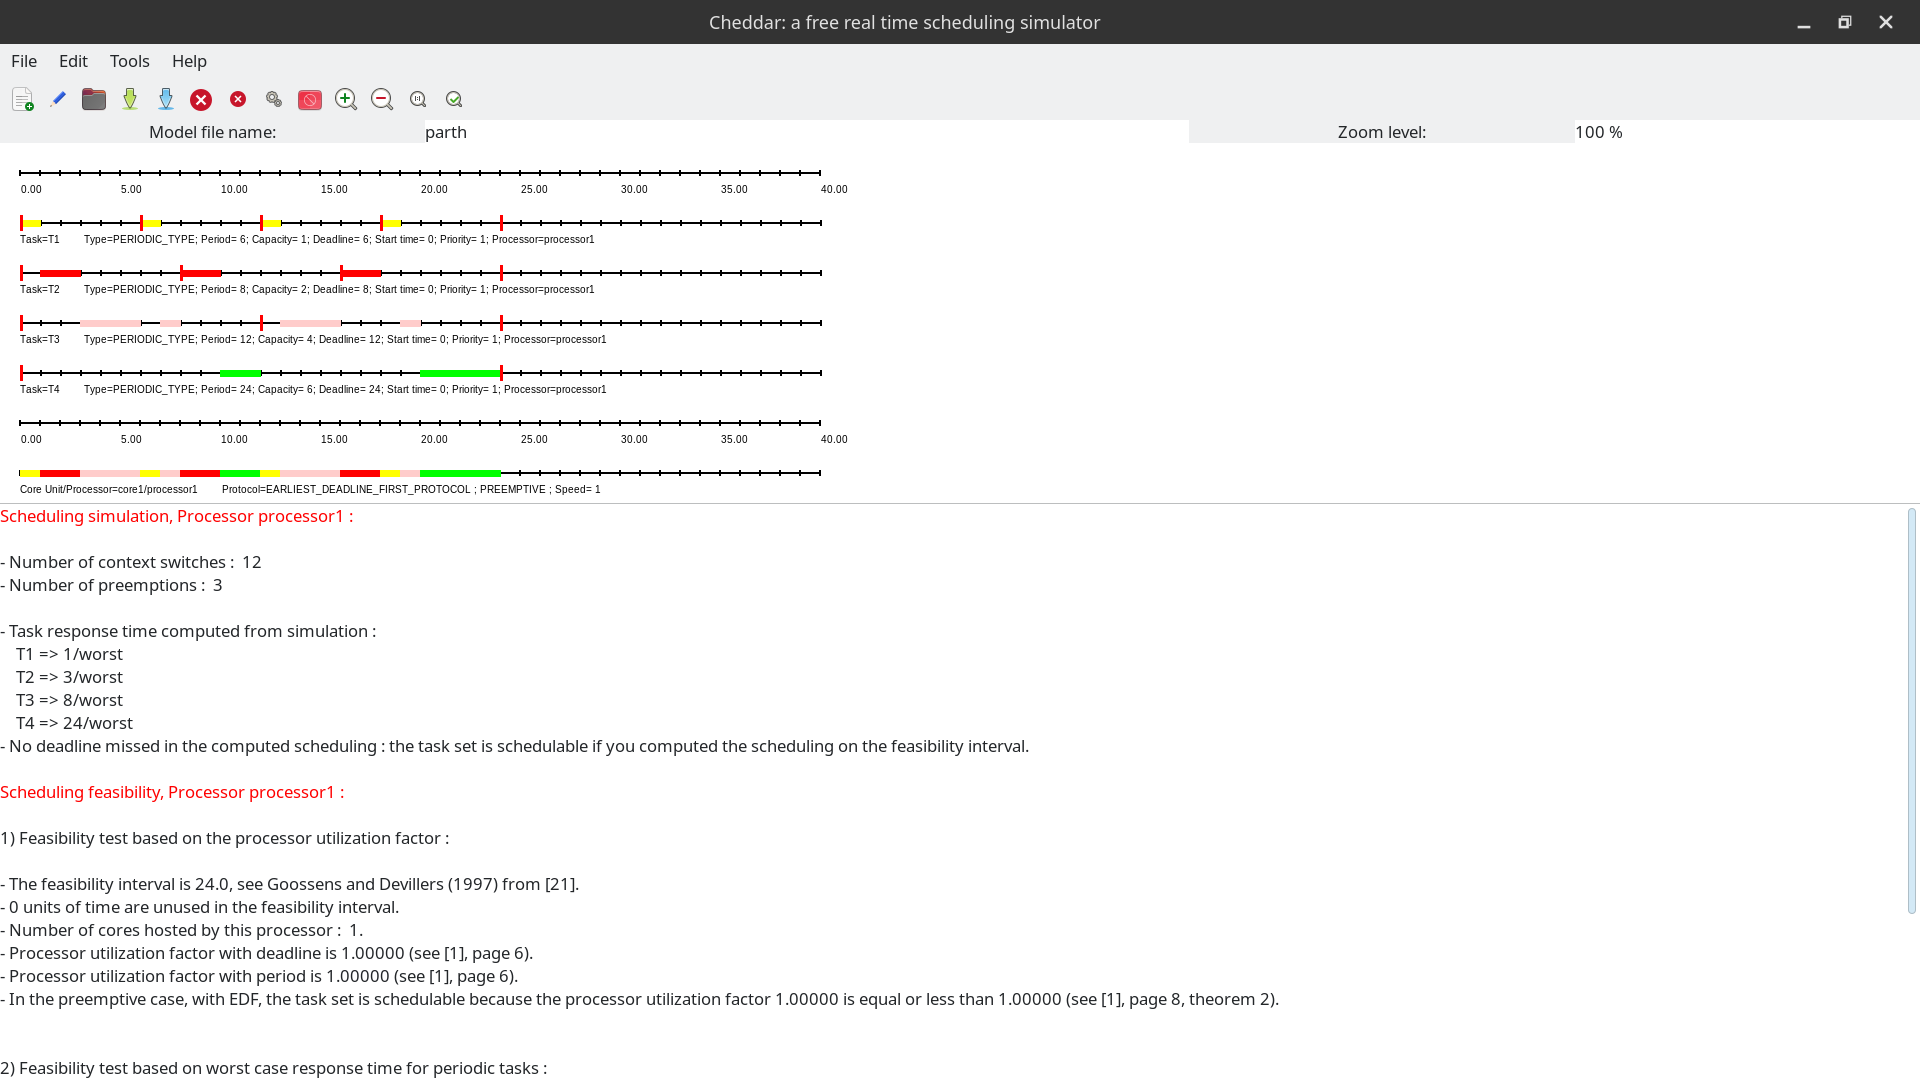
\includegraphics[scale=0.36]{figures/ex9_edf.png}
							                  \caption{Example 9, EDF analysis}
						                  \end{figure}
						                  \textbf{LLF Schedule}
						                  \begin{figure}[H]
							                  \centering
							                  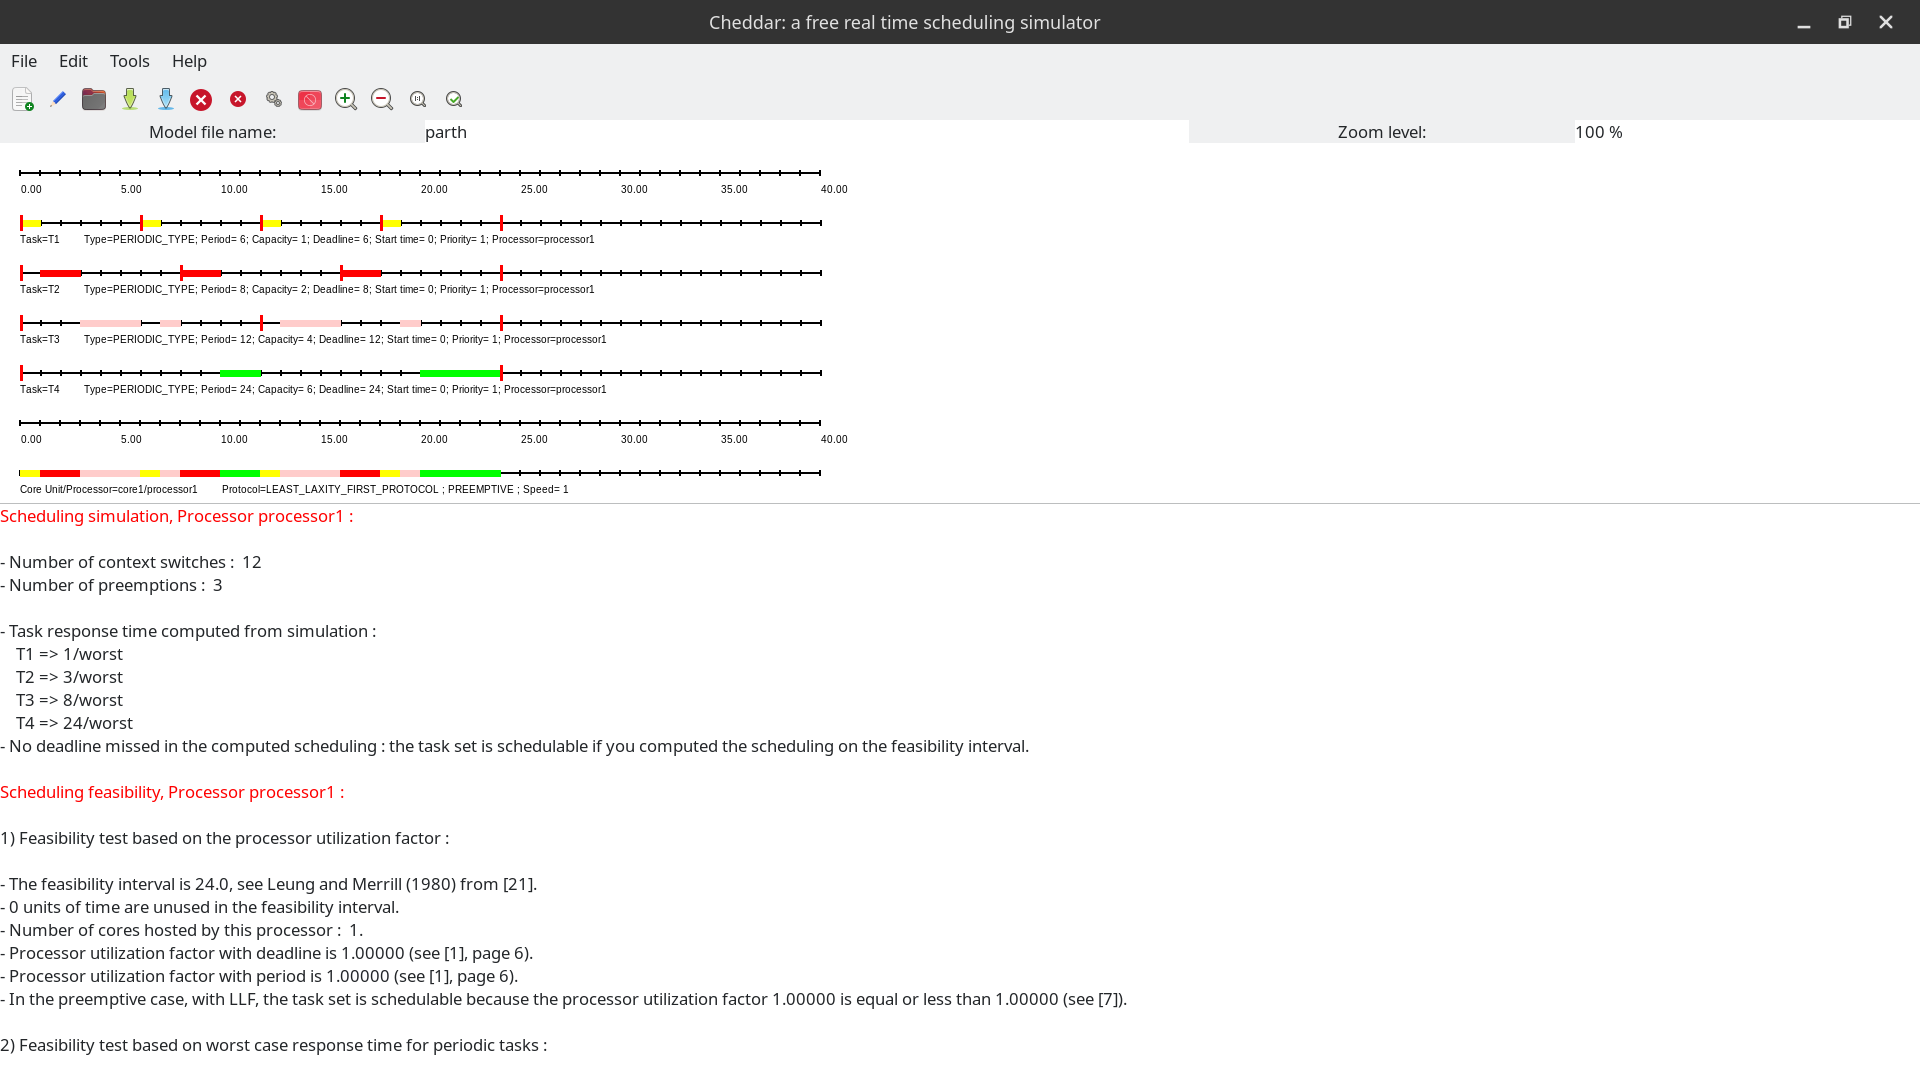
\includegraphics[scale=0.36]{figures/ex9_llf.png}
							                  \caption{Example 9, LLF analysis}
						                  \end{figure}
						            \item \textbf{Code Output:}\\
						                  \begin{verbatim}
****************
Example 9
C: 1 2 4 6
T: 6 8 12 24
D: 6 8 12 24

Task 0, WCET=1, Period=6, Utility Sum = 0.166667
Task 1, WCET=2, Period=8, Utility Sum = 0.416667
Task 2, WCET=4, Period=12, Utility Sum = 0.750000
Task 3, WCET=6, Period=24, Utility Sum = 1.000000

Total Utility Sum = 1.000000
LUB = 0.756828
RM LUB: Infeasible
Completion time feasibility: Feasible
Scheduling point feasibility: Feasible

(Period)
Total utility in EDF: 1.000000 Which is less than 1.0
EDF: Feasible
Total utility in LLF: 1.000000 Which is less than 1.0
LLF: Feasible
									\end{verbatim}
						            \item \textbf{Conclusion:}\\
						                  The Least Upper Bound (LUB) number is 0.756828, a figure that matches both in our own calculations and in the Cheddar software tests. However, we noticed that the CPU usage is really high, around 99.67\%, and this level of usage is also reflected in the Cheddar analysis when we look at the timing of tasks and their deadlines.\\

						                  Because the LUB value is higher than the actual CPU usage RM\_LUB would fail in the test, but all our checks for nessesarry and sufficient tests Completion time and Scheduling point feasibility shows that the tasks are feasible with RM schedule. This means we set up our tasks in a way that they can all get done within their set times without overloading the CPU. And we can confirm the results of no deadline miss in the cheddar.\\

						                  The output of code for the EDF and LLF shows that these set of tasks are schedulable with EDF and LLF as the utilization is less than or equal to 100\% and we can see in the cheddar output that EDF and LLF are indeed feasible. Cheddar shows that in EDF or LLF, no deadlines are missed and therefor these set of tasks are feasible for EDF and LLF.\\

						                  So, these task are schedulable by RM, EDF or LLF Policy.

					            \end{enumerate}
				      \end{enumerate}


				      \addcontentsline{toc}{subsection}{C}
				\item \Q Does your modified Feasibility code agree with Cheddar analysis in all 5 additional cases? Why or why not? And why edf and llf do not miss deadlines in the example while RM misses the deadline
				      \A
				      \textbf{Output of the cheddar and the code is equally right and it satisfies the feasible tests.}\\

				      Now, let's Take example Example 8 in which RM is Infeasible and EDF and LLF are feasible,\\
				      \begin{table}[H]
					      \centering
					      \caption{Tasks Parameters}
					      \label{tab:example}
					      \begin{tabular}{l c c c} % alignment of each column: l=left, c=center, r=right
						      \hline
						      Task  & Capacity  & Period     & Deadline   \\ \hline
						      $S_1$ & $C_1$ = 1 & $T_1$ = 2  & $D_1$ = 2  \\
						      $S_2$ & $C_2$ = 1 & $T_2$ = 5  & $D_2$ = 5  \\
						      $S_3$ & $C_3$ = 1 & $T_3$ = 7  & $D_3$ = 7  \\
						      $S_4$ & $C_4$ = 2 & $T_4$ = 13 & $D_4$ = 13 \\
						      \hline
					      \end{tabular}
				      \end{table}



				      Given the task characteristics, let's analyze why RM (Rate Monotonic) scheduling might miss deadlines, even though the total utilization is below 1, indicating that EDF (Earliest Deadline First) and LLF (Least Laxity First) would be feasible.\\

				      Rate Monotonic (RM) Scheduling
				      In RM scheduling, tasks are assigned priorities based on their period lengths, with shorter periods getting higher priority. Accordingly, the priorities here would be:\\

				      Highest Priority: Task 0
				      Lower Priorities: Task 1 $>$ Task 2 $>$ Task 3\\

				      \textbf{Analysis for Deadline Miss}\\
				      To understand where a deadline miss occurs in RM scheduling, we'll examine the scheduling timeline closely.

				      Initial Phase (First 13 Units of Time): The crucial point to examine is the first 13 units of time, which is the period of the lowest priority task (Task 3). During this time, Task 0 will execute 6 times, Task 1 will execute 2 times, and Task 2 will execute once, before Task 3 gets a chance to execute its 2 units of work.
				      Task 3 Deadline Miss: Task 3, having the lowest priority, can potentially miss its deadline due to the following scenario:\\
				      Task 0, 1, and 2 collectively require\\
				      6 $\cdot$ 1 + 2 $\cdot$ 1 + 1 $\cdot$ 1 = 9,\\
				      9 units of time within the first 13-time units, excluding overheads and assuming they preempt Task 3 whenever they become ready.\\

				      Task 3 requires 2 consecutive units of time to execute. However, due to its lower priority, its execution can be delayed by the execution of higher-priority tasks. If any of the higher-priority tasks become ready during Task 3's execution window, Task 3 will be preempted, potentially leading to a situation where it cannot complete its 2 units of execution before its deadline at time 13.\\

				      \textbf{Observation}\\
				      The deadline miss for Task 3 under RM scheduling arises because RM does not account for the actual deadlines when assigning priorities; it only considers the periods. This approach can lead to inefficiencies when lower-priority tasks have long execution times or when the distribution of task executions leads to higher-priority tasks preempting lower-priority tasks close to their deadlines.\\

				      \textbf{Why EDF and LLF Do Not Miss Deadlines}\\
				      EDF: Prioritizes tasks based on their absolute deadlines. Even if Task 3 has a longer period, as its deadline approaches, it would gain priority over other tasks, ensuring it gets CPU time to meet its deadline.
				      LLF: Prioritizes tasks based on their remaining laxity (time until deadline minus remaining execution time). As Task 3's deadline approaches without it having executed, its laxity decreases and I executes first instead of missing the deadline.




			\end{enumerate}


	\end{enumerate}

	\section{Question 5}
	\begin{enumerate}
		\item[] \Q [30 points] Read Chapter 3 of the textbook.
			\begin{enumerate}
				\addcontentsline{toc}{subsection}{A}
				\item \Q Briefly describe and provide 3 constraints that are made on the RM LUB derivation and 3
				      assumptions as documented in the Liu and Layland paper and in Chapter 3 of the text.
				      Describe whether you think each is reasonable for actual practice or whether you think each is only applicable to and idealized model of practice.
				      \A

				      The Liu and Layland paper, a seminal work in real-time systems, introduces the Rate Monotonic (RM) scheduling algorithm and its Least Upper Bound (LUB) for CPU utilization. In this context, certain constraints and assumptions are made for the derivation of the LUB, and understanding these is crucial for applying the theory to practical scenarios.


				      \begin{enumerate}
					      \item  \textbf{Constraints in the RM LUB Derivation}
					            \begin{enumerate}
						            \item \textbf{Fixed Task Set with Harmonic Periods} The derivation initially considers only two tasks, under the assumption that if the LUB can be proven for two tasks, it extends to any number of tasks. This simplification assumes a fixed task set, which might not always be the case in dynamic systems where tasks can vary over time.
						            \item
						                  \textbf{Worst-Case Execution Time (WCET) Overlap:} It's assumed that the WCET does not perfectly fit within the task periods, allowing for some overlap. This constraint is realistic as it accounts for the variability in execution times and the potential for tasks to run longer than their allocated time slots.
						            \item
						                  \textbf{Minimum Interference (I=1):} The derivation assumes that the least upper bound for utilization occurs when higher-priority tasks interfere with lower-priority tasks by the minimum amount possible, exactly once. This assumes a very idealized scenario where task executions are perfectly aligned to minimize interference while still adhering to priority constraints.
					            \end{enumerate}

					      \item  \textbf{Assumptions in the RM LUB Derivation}
					            \begin{enumerate}
						            \item \textbf{Task Independence:} Tasks are assumed to be independent of each other, with no synchronization or shared resources. This assumption simplifies the analysis but might not hold in complex systems where tasks often interact or share resources.
						            \item
						                  \textbf{Static Priority Scheduling:} RM scheduling assigns static priorities based on task periods, with shorter periods implying higher priorities. This assumption neglects the potential need for dynamic priority adjustments in response to runtime conditions.
						            \item
						                  \textbf{Complete Utilization of CPU:} The derivation assumes that the system aims to maximize CPU utilization without overloading the processor. In practice, this might not always be desirable as systems might prioritize responsiveness or power efficiency over maximizing utilization.

						                  The LUB for utility increases as the potential for task schedulability under RM becomes more constrained. When I is minimized, it suggests an optimal frequency of interference that allows for the highest possible utility without violating the schedulability constraints of RM. In other words, minimizing I maximizes the efficiency of task scheduling under RM, allowing for the highest total utilization (or LUB) where tasks can still be guaranteed to meet their deadlines.
					            \end{enumerate}
					      \item Applicability to Practice
					            \begin{enumerate}
						            \item \textbf{Fixed Task Set and WCET Overlap:} These constraints are relatively reasonable in systems where the task set is known a priori, and tasks have been analyzed for their worst-case execution scenarios. However, dynamic systems where tasks can change or where execution times are highly variable might not fit well within these constraints.

						            \item \textbf{Minimum Interference:} While aiming for minimal interference is ideal, in practice, the actual interference pattern can be much more complex due to the unpredictable nature of task executions and system load. This assumption serves more as a theoretical ideal than a practical expectation.

						            \item \textbf{Independence and Static Priority:} These assumptions simplify analysis but might not reflect the complexity of modern systems where task interactions and the need for adaptability can't be overlooked. Static priorities might not suffice in systems requiring more flexible scheduling approaches to respond to changing conditions.
					            \end{enumerate}

				      \end{enumerate}


				      \addcontentsline{toc}{subsection}{B}
				\item \Q Finally, list 3 key derivation steps in the RM LUB derivation that you either do not
				      understand or that you would consider “tricky” math. Attempt to describe the rationale
				      for those steps as best you can do based upon reading in Chapter 3 of the text.r deterministic and compare your results.
				      \A
				      Case 1 represents that the utilization monotonically decreases with increasing C1 when T1$>$T2.
				      Case 2 represents that the utilization monotonically increases with increasing C1 when T1$>$T2.
				      RM policy assumes that T2 $>$ T1.

				      \begin{enumerate}
					      \item In the derivation, we want to determine the utility when C1 exceeds or is less than the critical time zone. It is mentioned that is determined by subtracting case 1 and case 2 utility data with varying T2 and C1. Exactly how it is achieved was not clear. According to our understanding, derivation is a mathematical approach for studying and understanding the relations between the parameters in utility for different situations. Finding the in which the system can function at the same degree of utility is the aim, since it offers important information about
					            whether real-time scheduling is feasible or not.
					      \item It is mentioned that the cases are valid only when services intersect and this can occur only when C1 is equal. If C1 is not equal, it implies that there is no common critical instant where the utility expressions for Case 1 and Case 2 intersect. In such a scenario, the analysis of the utility equation might not yield a valid LUB for the system's utility. It was difficult to understand this case.
					      \item The derivation also assumes that the least upper bound for utilization occurs when higher-priority tasks interfere with lower-priority tasks by the minimum amount possible, i.e. exactly one. Assumption made was unclear. The assumption is that the smallest possible value for I is 1, indicating that there is exactly one instance of S1 occurring during the execution of S2. This assumption simplifies the analysis and allows for the derivation of the least upper bound for utilization.
				      \end{enumerate}




			\end{enumerate}


	\end{enumerate}

	\section{Challenges Faced}
	\begin{enumerate}
		\item Understanding the key assumptions made in the derivation and the reason why these assumptions are necessary
		      was difficult to understand.
		\item Learning cheddar tool and getting used to it was initially challenging but later on was fun.
	\end{enumerate}


	\section{Conclusion}
	\begin{enumerate}
		\item We understood  the concept of the Cyclic Executive and its comparison with Linux POSIX RT threading and RTOS.
		\item Implemented and analyzed custom feasibility test code for different scheduling policies (RM, EDF, LLF) using Cheddar.
		\item Moreover, learned the constraints, assumptions, and derivation steps in Rate Monotonic (RM) Least Upper Bound (LUB) as mentioned in Chapter 3 of the textbook.

	\end{enumerate}

	\section{References}
	\begin{enumerate}
		\item ECEN 5623 Lecture slides material and example codes.
		\item REAL-TIME EMBEDDED COMPONENTS AND SYSTEMS with LINUX and RTOS, Sam Siewert John
		      Pratt (Chapter 3, 4 \& 5).
		\item Exercise 2 requirements included links and documentation.
	\end{enumerate}


\end{qanda}




\vfill
\hrule
\vspace{0.5cm}
\pagebreak
\begin{appendices}
	\section{C Code for the Implementation}
	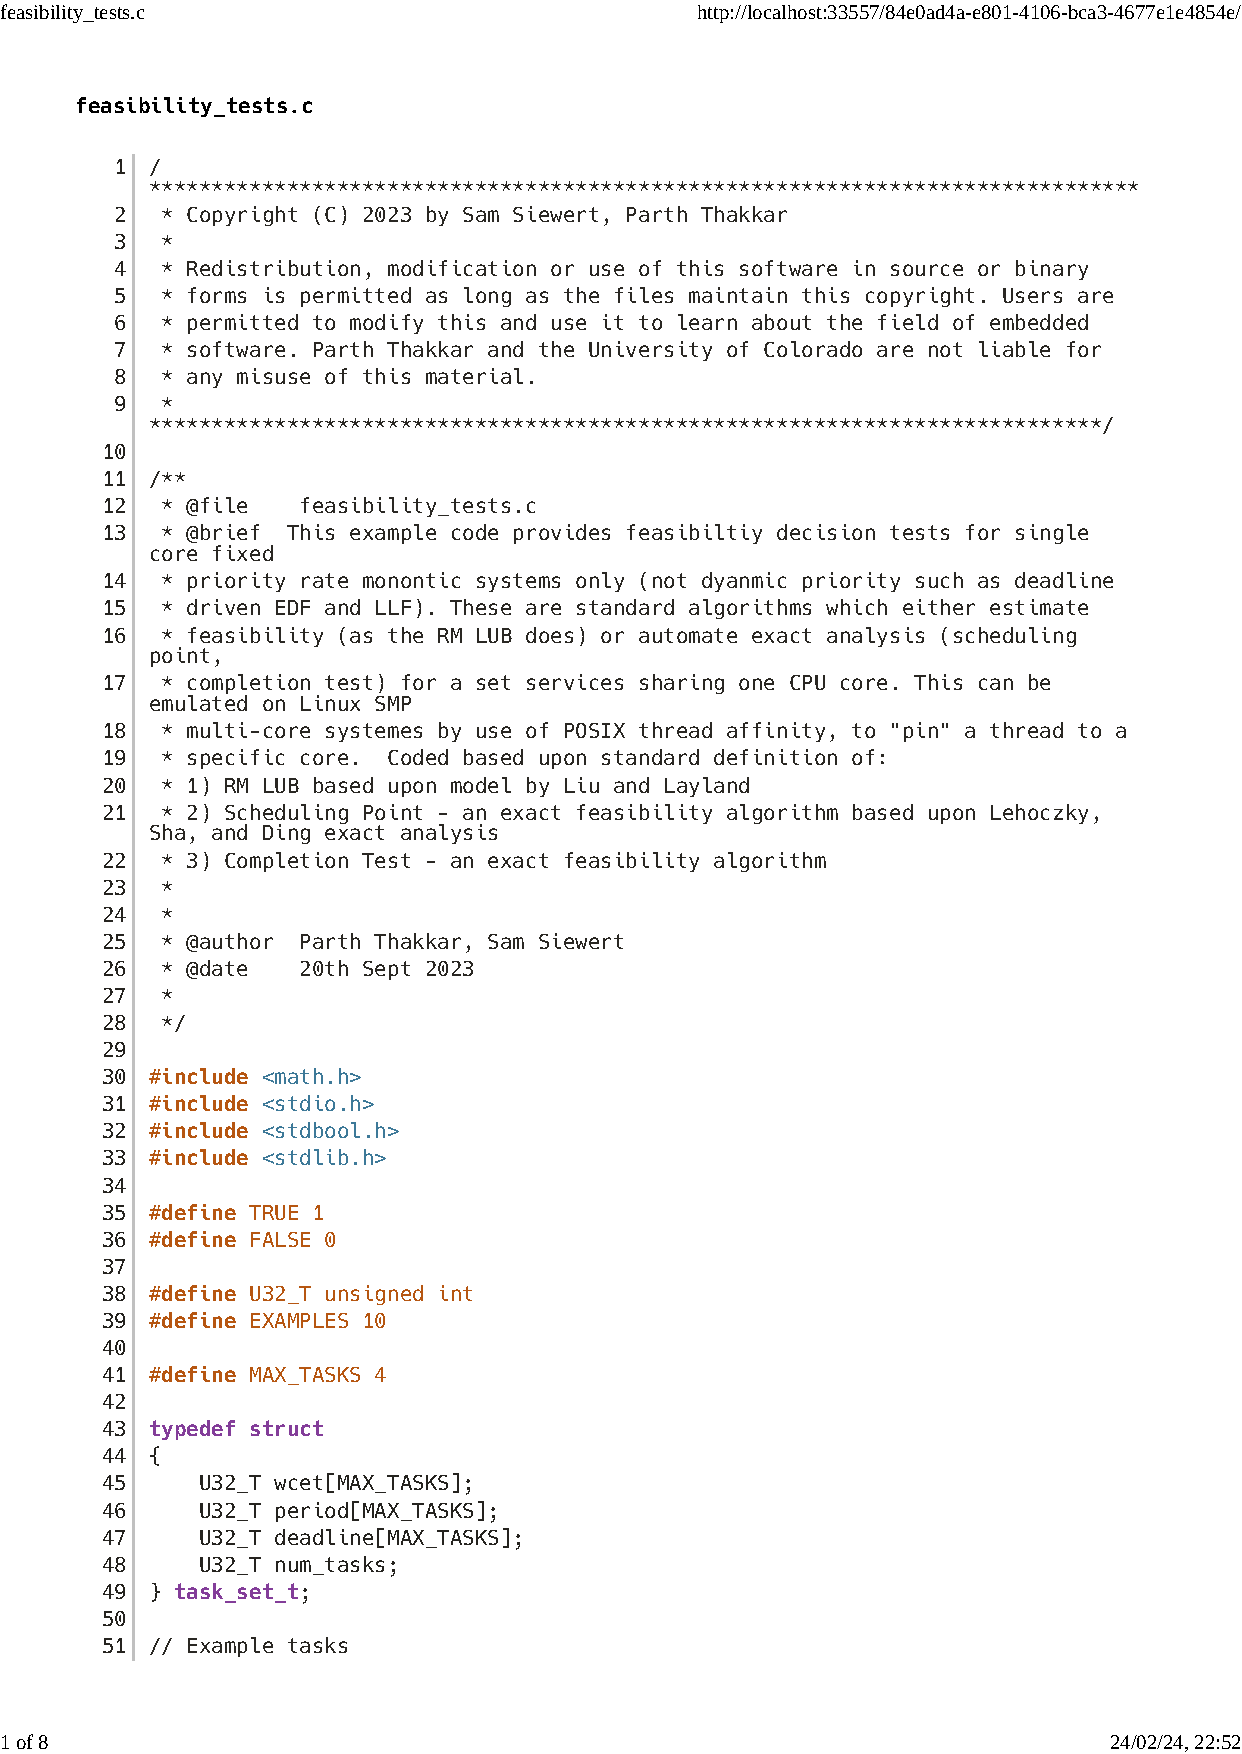
\includepdf[pages=-]{code/feasibility_tests.pdf}
\end{appendices}


\vspace{1cm}
\hrule
\vspace{0.5cm}


%---------------------------------------------------------------------------
\end{document}
-
